

\chapter{Segmentation of Liver Tissue in computed tomography} \label{SegSemantic}

\section{Introduction}

As explained in the chapter \ref{liverCancer}, the liver is an
organ with a key function in the human body. Being a soft organ, it
presents a large variation in shape among the population (inter-patient
variation), and can also be subject to deformations due to respiratory
and heart motions in case of multiphasic acquisition after injection of
contrast agents (intra-patient variation).\\
On computed tomography images, the intensities of the liver itself and
those of nearby organs (heart, spleen, stomach) are very similar. The
images are often acquired after the injection of contrast agents to
offer critical information (e.g. \emph{wash-in/wash-out}). Nonetheless,
the acquisition protocol may differ among the institutions (type of
contrast agent, moments of injection, injection rate, \ldots{}) and the
results often differ with the patient characteristics (e.g. blood flow).
Moveover, the liver can easily be affected by diseases such as
cirrhosis, and is often the site of either primary or secondary cancers
with varying contrast levels (hyper-/hypo-intense tumors, peritumoral
enhancement) and shapes (non-smooth margins, hypoattenuating halos,
\ldots{}). All these reasons cause the automatic or semi-automatic
segmentation of the liver and its structures to be challenging.

%In this section, we will briefly present the medical value brought by an automatic segmentation of the liver and its internal structures, before raising the issue related to the scarcity of publicly available liver CT datasets with associated experts annotations. 
%We will then introduce the classical semantic segmentation techniques based mainly on traditional computer vision and machine
%learning methods, before presenting the improvements brought by the deep learning which has the ability to extract relevant features in a data-driven manner.
%Finally, we will expose our semantic segmentation experiments where the best performances were obtained by stacking several specialized networks with temporal images as input.

In this section, we are first covering the different publicly available datasets as long
as the different challenges launched to increase interest in liver
semantic segmentation. We are then investigating the first methods
developed to perform the semantic segmentation of the liver and/or liver
tumors, before presenting most recent advances brought by deep learning (DL).
The hand-crafted feature based methods were often guided by manual interactions,
and commonly implemented engineered features whereas deep learning
allowed relevant features to be learned directly from the input data.
Finally, we  expose our semantic segmentation experiments where 
the best performances were obtained by stacking several 
specialized networks with dynamic contrast-enhanced images as input.


%{Medical value brought by liver tissue segmentation}
The automatic segmentation of the tumors allows the computation 
of the entire tumor volume, which corresponds to a better predictor when
compared to the diameter only, according to the \emph{Response
	Evaluation Criteria in Solid Tumor} (RECIST) standard \cite{Eisenhauer2008, Ye2017}. A precise
volumetric segmentation of both the liver and its tumors is a
prerequisite in case of treatment planning, (\emph{TARE}, \emph{TACE,
	percutaneous thermal ablation, radiotherapy surgical resection,\ldots{}}) especially to adjust the treatment procedures to the volume of the lesions\cite{Al-Nahhas2014, Yamada1983, Albain2009, Rossi96}. Associating liver and tumors
segmentation allows the computation of the \emph{tumor burden}\footnote{proportion of the liver affected by cancer}, which
has an importance in case of surgical resection, or when estimating the
efficiency of a given treatment \cite{Nordlinger1996, Jagannath1986, Gobbi2004, Bauknecht2010, Bornemann2007, Heussel2007, Kuhnigk2006, Puesken2010}.

%{Problems related to the lack of data}

Relying on human expert
delineations currently corresponds to the most common way to assess
segmentation methods \cite{Bilic2019}, although it does not correspond 
to a true gold standard \cite{Heimann2009} and often requires several experts to segment the
different structures for reducing the operator-dependent bias \cite{Echegaray2015, Moltz2009}.\\
In order to compare digitally obtained segmentations with the expert
outputs, different metrics have been implemented over time (see
``\emph{Semantic Segmentation Metrics}'' in Appendix). However, as
explained above, manually segmenting the liver and its different
structures is a tedious, time-consuming (up to 90 minutes per patient
\cite{Gotra2017}) and operator-dependent task, as seen in the figure \ref{interobserver_var}.
Furthermore, the constitution of an open database needs to respect
several ethical aspects, and the patient data privacy. This is the main
reason why only a small number of samples have been publicly released
over time.

\begin{figure}[!h]
	\centering        
	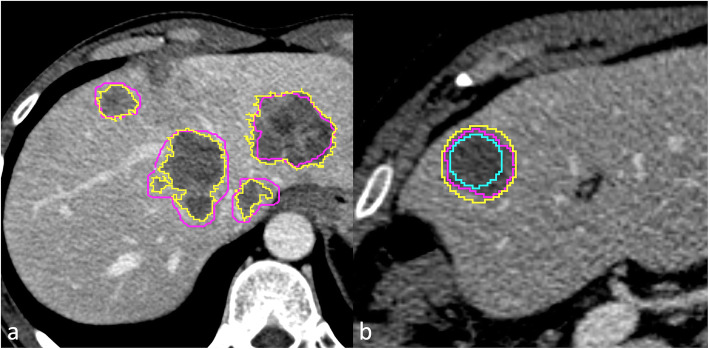
\includegraphics[width=0.7\linewidth]{./images/interObs1}
	\caption{Interobserver variability: For each metastasis, the whole lesion volume and the largest axial cross-section were segmented by two readers. a Purple line (reader 1) versus yellow line (reader 2) contouring. The largest two-dimensional (2D) region of interest (ROI) of the main lesion was confronted with two circular ROIs, one inside the metastasis and one outside it. b Purple line (reader 1) 2D versus yellow line (smallest circular ROI inclusive of the whole lesion) versus azure line (largest circular ROI completely inside the lesion). \textbf{©Rizzetto et al. \cite{Rizzetto2020}}}
	\label{interobserver_var}
\end{figure} 

\section{Publicly available datasets \& open challenges}

Up to today, and compared to other organs (brain, breast, lung) \cite{GrandChallenge}, only
a small number of computed tomography images datasets have been publicly
available for liver tissue segmentation purposes. A table presenting
details of the publicly available datasets can be found in the table \ref{publicly_available_datasets}.

\renewcommand{\arraystretch}{2}
\setlength{\tabcolsep}{8pt}
\newgeometry{top=5mm, left=5mm, right=5mm, bottom=10mm, footskip=5mm, headsep=10mm}
\begin{landscape}
	\scriptsize
	\begin{longtable}{l|p{1cm}p{1cm}p{1.5cm}p{1.5cm}p{2cm}p{1.2cm}p{2cm}p{2cm}p{2cm}p{2cm}p{1cm}p{2cm}}\toprule
		\textbf{Name} &\textbf{\#Cases} &\textbf{Liver GT} &\textbf{Tumor GT} &\textbf{Tumor Type} &\textbf{Other GT} &\textbf{\#Experts} &\textbf{Volume size\newline(pixels)} &\textbf{Voxel size \newline (mm)} &\textbf{Challenge} &\textbf{Hidden\newline Cases} &\textbf{Phases} \\\midrule
		\textbf{3Dircad-01} &\textbf{20} &true &true &Undefined &Blood vessels&1 &axial: 512x512\newline z : 74 - 260&axial:0.56 - 0.87\newline z: 1 - 4&- &- &Undefined \\
		\textbf{3Dircad-02} &\textbf{2} &true &true &FNH &- &1 &axial: 512x512\newline z: 167 - 219&axial: 0.96\newline z: 1.8 - 2.4&- &- &1 AR\newline 1 PV\\
		\textbf{Sliver07} &\textbf{30} &true &true &Undefined &- &1 &- &axial: 0.55 - 0.8\newline z: 1 - 3&MICCAI07 &10 &PV \\
		\textbf{MIDAS} &\textbf{4} &false &true & Undefined &- &5 &- &- &- &- & Undefined \\
		\textbf{LITS} &\textbf{131} &true &true &Undefined &No &3 &axial: 512x512\newline z: 42 - 1026&axial:0.56 - 1\newline z: 0.45 - 6&MICCAI17\newline ISBI 2017&70 &Undefined \\
		\textbf{TCIA} &\textbf{97}\footnote{CT and/or MR images volumes} &false &false &HCC &No &- & axial:512x512 \newline z: 26 - 192 & axial: 0.58 - 0.98 \newline z: 0.8 - 5 &- &- &mixed\\
		\textbf{CHAOS} &\textbf{40} & true &false &\textbf{Healthy \newline Livers}&No &3 &axial: 512x512\newline z: 77 - 105&axial: 0.7 - 0.8\newline z: 3 - 3.2&ISBI 2019 &- &PV \\
		\textbf{ImageClef Liver}&\textbf{50} &true &true\newline (Bounding Box) &- &No &- & x: 190- 308\newline y: 213-238\newline z: 41 - 588& axial: 0.68 - 1.01 \newline z: 0.40 - 2.5 &ImageClef 2015 &10 & Undefined \\
		\bottomrule
		\caption{Publicly available datasets}\label{publicly_available_datasets}
	\end{longtable}
\end{landscape}
\renewcommand{\arraystretch}{5}
\newgeometry{vmargin={15mm}, hmargin={30mm,30mm}}   % set the margins 

Some of the available datasets have been launched by medical-related
institutions. IRCAD (\emph{Research Institute Against Digestive Cancer})for example, provided both 3DIrcadb sets \cite{3DIrcadB}, with the first containing 20 abdominal CT
scans, where 15 of the patients suffered from liver tumor, and the
second containing only 2 CT scans with patients suffering from FNH
(\emph{Focal Nodular Hyperplasia}).
The \emph{National library of Medicine} (NLM) offered the MIDAS dataset
containing annotated pathological CT scans from 4 patients \cite{MIDAS} whereas the cancer imaging archive (TCIA)
proposed a set of 97 unlabeled volumes from patients suffering from
hepatocellular carcinoma (HCC) \cite{Clark2013}. \\
Thanks to the different segmentation challenges launched throughout the
time, some other sets have been provided and offered real benchmarks.
The \emph{Segmentation of the Liver} (Sliver'07) was organized in
conjunction with MICCAI 2007 and offered 40 CT volumes \cite{VanGinneken2007}, where 30
volumes were available during the challenge, and 10 hidden cases were
used to evaluate the proposed methods. In 2015 the Image Clef challenge
offered 50 CT scans with expert annotations \cite{ImageClef}, whereas 201 volumes have been provided by the organizers
of both ISBI and MICCAI in 2017 for the \emph{Liver Tumor Segmentation}
(LITS) benchmark \cite{Bilic2019}. In 2019 the organizer of ISBI
further granted access to 40 cases for the \emph{Combined (CT-MR)
	Healthy Abdominal Organ Segmentation} (CHAOS)\cite{CHAOS}.

In these different datasets, the volumes were annotated by one or
multiple experts, with predominantly pixel-wise delineations of the
areas of interest (the ImageClef dataset is the only one with bounding
box annotations for the lesions). Only one annotation volume per case is
given which is designed to translate the consensus among the experts,
however, the inter-expert variations can not be correctly caught by this
format. Moreover, most of the available databases present heterogeneous
data in terms of geometry (number of slices per patient, volume size,
resolution), pathology (the number of lesions per volume in the LITS
dataset goes from 1 to more than 70) and regarding the
acquisition protocols (e.g. the acquisition phase is undefined for the
LITS data where arterial and portal venous volumes are mixed up).\\

%\begin{figure}[!ht]
%	\centering
%	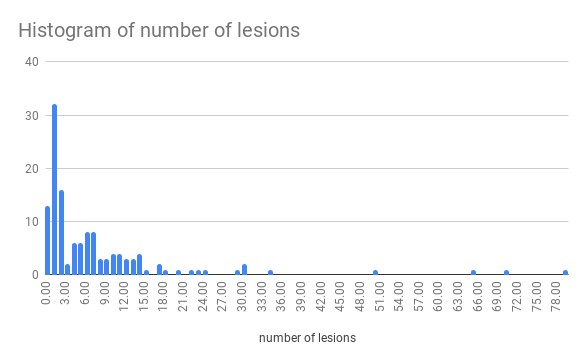
\includegraphics[width=0.7\linewidth]{images/image11}
%	\caption{Histogram of the number of lesions per patient in the LITS dataset}
%	\label{NumberOfLesionsLits}
%\end{figure}
%The limited access to data and the heterogeneity present in the publicly
%available datasets render thus the liver tissue segmentation task very
%challenging.

\section{Hand-crafted feature based semantic segmentation methods}

A total of 61 studies performing either the segmentation of the liver and/or its tumors 
were reviewed to introduce the different hand-crafted feature based segmentation methods. 
Even though the majority of the studies 
 combined several concepts to perform the segmentation, they were classified 
 based on the algorithm using the most domain-specific knowledge \cite{Moghbel2018}.
The reviewed studies included in this section were initially dedicated
 to the liver segmentation \footnote{48 over the 61 reviewed studies were only dedicated to
 the segmentation of the liver} since this task received initially more interest from the researchers than the liver tumors segmentation task. However, 
 the majority of the detailed methods can also address the semantic 
 segmentation of liver tumors or the segmentation of other abdominal 
 organs\footnote{6 studies among the 61 retained ones performed both the 
 segmentation of the liver and its tumors, whereas 7 others segmented both the liver and other abdominal organs}. \\
The first methods that have been used for the semantic segmentation of
liver tissue relied mainly on computer vision and machine
learning methods. In most of the cases, prior anatomical knowledge about
the intensity, the shape or the position of the liver is incorporated in
the process. The different methods are supported by several pre- and
post-processing steps, and may require one or multiple interactions with
experts.\\
Among the most utilized methods, we will first present those based on
the intensity of the voxels, before mentioning the ones requiring manual
interactions such as region growing or graph-theory based methods. We will 
then introduce the geometric deformable models that can be exploited to add 
local constraints, before introducing methods 
requiring prior shape knowledge such as
probabilistic atlases (PA) or statistical shape models (SSM).
Finally, we will mention the different studies that combined the
aforementioned methods with the addition of machine learning based steps.
%The studies included in this section were applied on the segmentation of either the liver alone, its potential tumors, or both, however we decided to separate them based on the used methods instead of focusing on the segmentation task, since the majority of the mentioned methods can fit both the tasks, but they were initially dedicated to the segmentation of the liver 

\subsection{Image Intensity based methods}

Some studies decided to first rely on the gray level distribution of
the liver in the training images to get an initial segmentation during
the inference, before applying a refinement step consisting on active
contours, region growing, or morphological techniques with anatomical
constraints.\\
Lim et al. \cite{Lim2004, Lim2005, Lim2006}, combined prior-knowledge such as the location of the liver
and its intensity distribution with active contours to segment the
liver. The rough estimation is determined via thresholding and
morphological operations in a multiscale fashion. K-means clustering is
applied to remove unwanted tissues from the candidate area. Active
contour, as described later, is then implemented to refine the liver boundary by first
detecting the boundary between liver and adjacent organs.
The segmentation pipeline is depicted in the figure \ref{IntensityBasedLim}.

\begin{figure}[ht!]
	\centering
	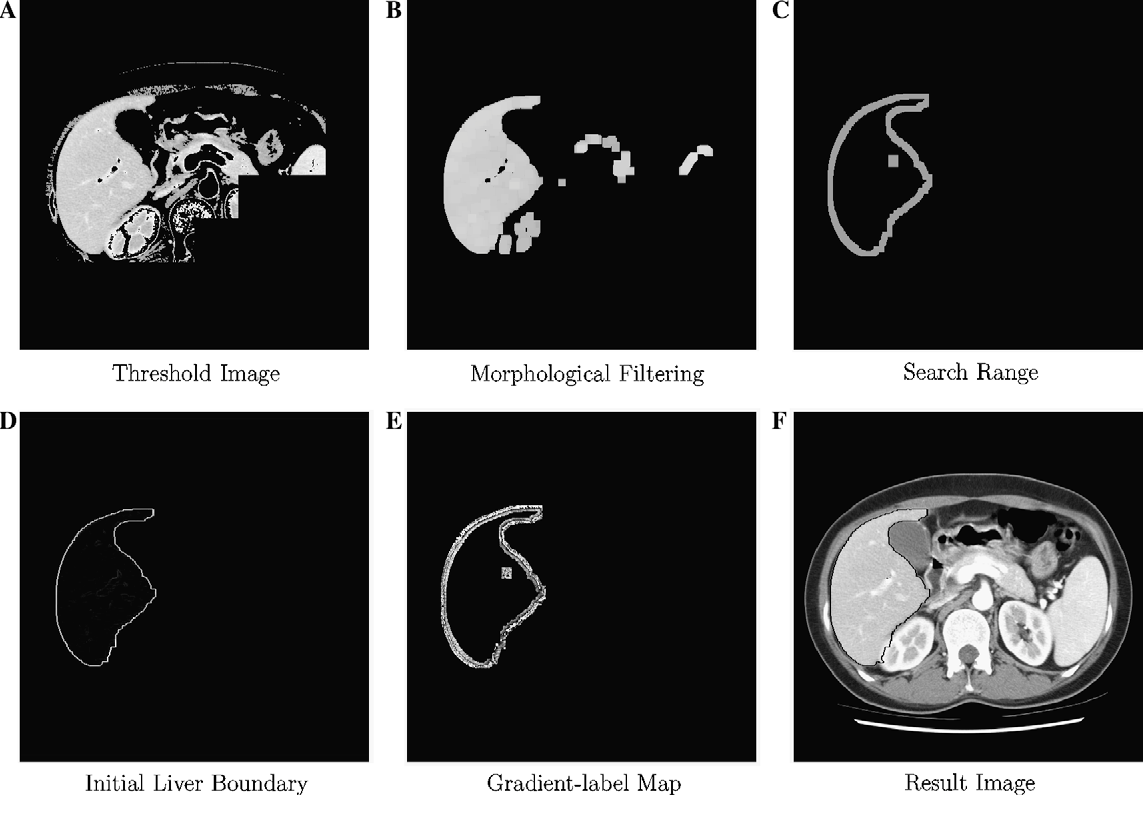
\includegraphics[width=0.7\linewidth]{images/Lim2006_Fig14}
	\caption{Intensity based liver segmentation workflow used by \textbf{©Lim et al.  \cite{Lim2006}}}
	\label{IntensityBasedLim}
\end{figure}

Lee et al. \cite{Lee2003}, proposed a multimodal contextual neural network using
pixel intensity and neighborhood dynamic to get a rough liver
segmentation. The refinement step is performed using fuzzy rules based
on prior knowledge such as location or textural properties.
Liu et al. \cite{Liu2005}, developed a method to segment the liver by first detecting the potential
contour implementing a Canny Edge detector algorithm, modified by the
template liver position obtained via thresholding. A Gradient Vector
Flow (GVF) field computation is used by the snake algorithm to obtain an
accurate liver boundary detection. The final segmentation is obtained
semi-automatically by asking the user to select the slices where the
segmentation gave accurate results, and propagate this segmentation
iteratively to adjacent slices. An example is depicted in the figure \ref{LiuGVF}.
\begin{figure} [ht!]
	\centering
	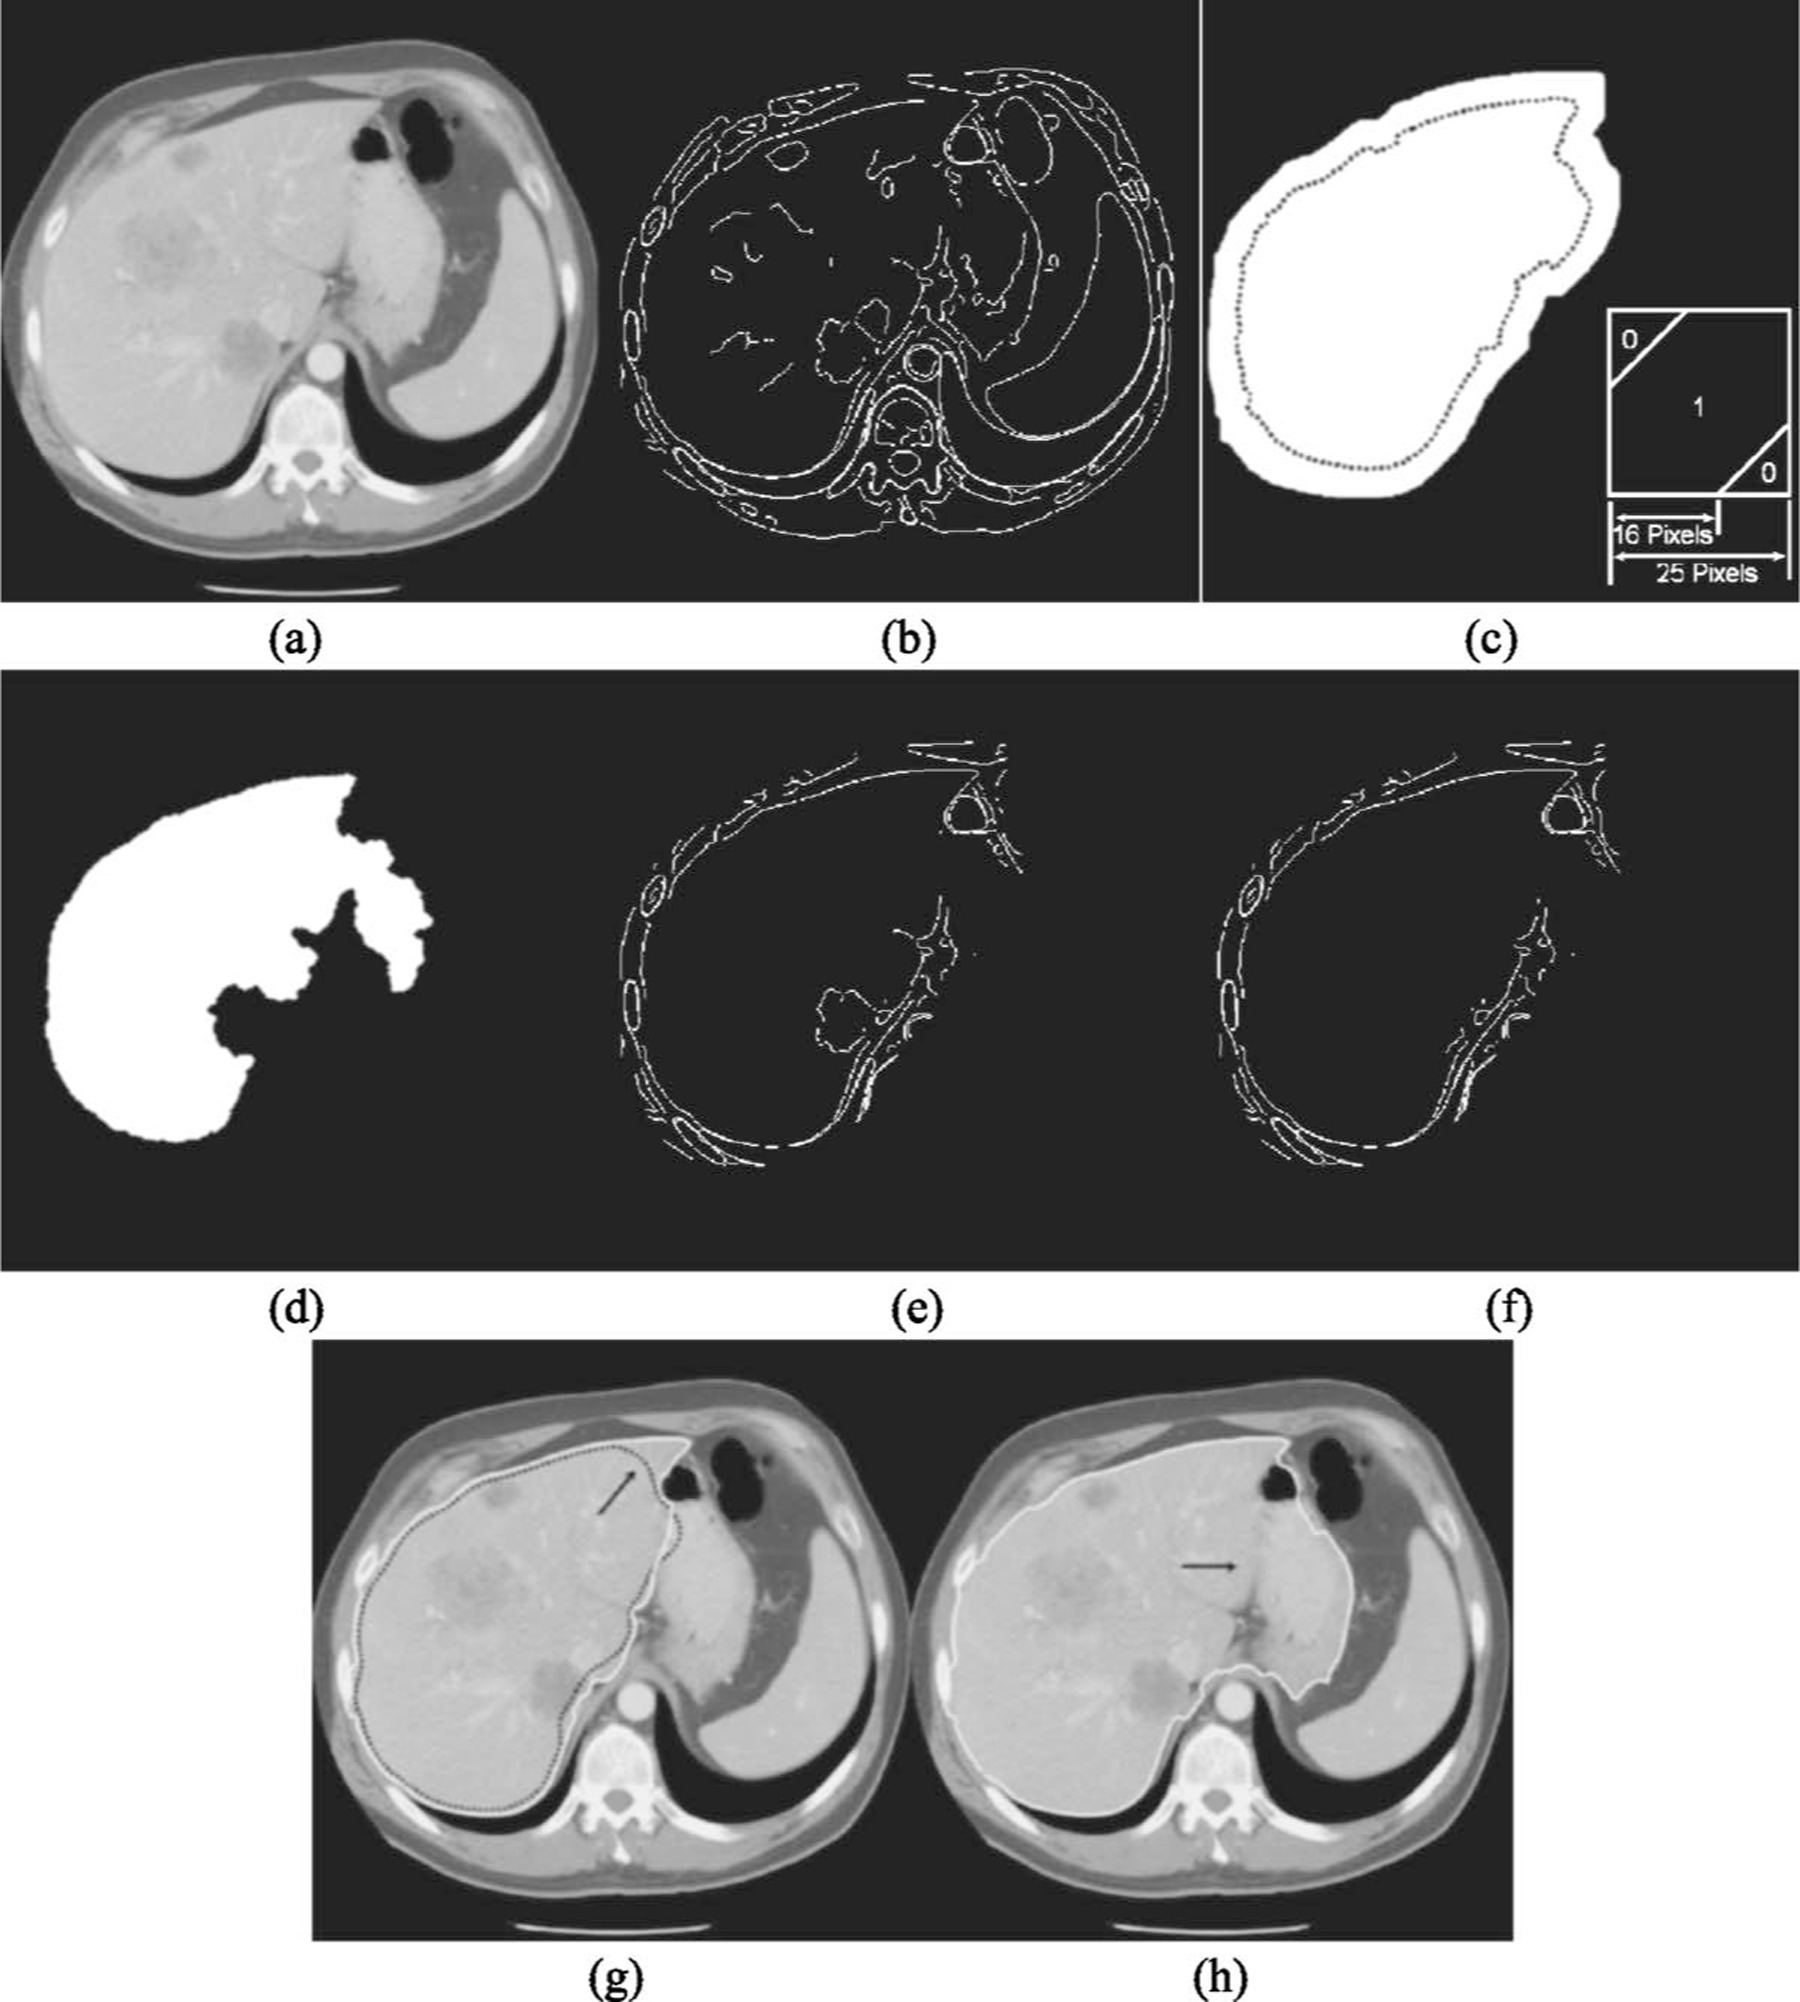
\includegraphics[width=0.6\linewidth]{images/Liu2005_Fig6}
	\caption{Liver segmentation as described by \textbf{©Liu et al. \cite{Liu2005}} : (a) Original image to be segmented, (b) Initial edge map (c) Dilated version of the neighboring slice mask (SSE in right lower corner) (d) The liver template (e) Edge map after modification by the mask and the liver template (f) Final edge map after modification by the concavity removal algorithm (g) The original image overlapped with the final contour (white solid) (h) Leakage if GVF is not applied.}
	\label{LiuGVF}
\end{figure}



Seo and Park \cite{Seo2005} 
combined thresholding techniques and morphological operations to obtain
a final liver segmentation. Specific filters are firstly used to smooth the
distribution and reduce the noise. Adaptive multi-modal threshold is
then applied to find the intensity range of the contrast enhanced liver.
The left partial histogram threshold (LPTH) algorithm is then
implemented to detect the liver and remove neighboring organs, before
morphological operations are performed to refine the candidate ROI.
Kim et al. \cite{Kim2007}, obtained a rough segmentation of the liver by comparing the gray
level dynamic of the test patient with gray-level distributions obtained
from liver ROIs in the training dataset. The ROI is refined using
watershed transform followed by anatomical constraints such as the
presence of smooth boundaries.
Campadelli et al. \cite{Campadelli2009}, proposed a new fully automatic liver segmentation
technique. They first constrained the research by considering only the
area below the heart. Different organs are afterwards classified, in
particular the liver which corresponds to the biggest connected
component found between the different organs. The liver region is
further refined using a region growing method to ensure 3D consistency.
Foruzan et al. \cite{Foruzan2009}, computed the liver intensity range using
expected-maximisation (EM) algorithm, and applied thresholding operation
in a bounding box constrained by the position of the ribs and the heart
as illustrated in figure \ref{ForuzanFig3}. The final candidate region of interest is then
refined by anatomical constraints such as liver anatomy and assumed
intensity range.

\begin{figure} [ht!]
	\centering
	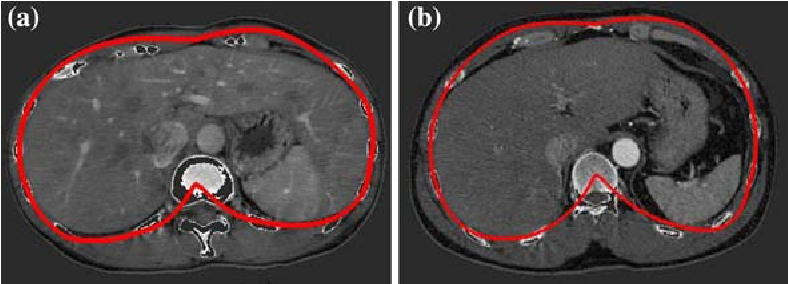
\includegraphics[width=0.7\linewidth]{images/Foruzan2009_Fig3}
	\caption{Estimation of the liver ROI based on the anatomical rib position as described by \textbf{©Foruzan et al. \cite{Foruzan2009}}}
	\label{ForuzanFig3}
\end{figure}


\subsection{Region Growing}

This set of methods
is based on the placement of an initial seed point/region and evolves
based on the image properties. As an example, Beck and Aurich \cite{Beck2007}, proposed to manually place seed points iteratively
until the entire liver is segmented by 3-D filling using non-linear
interpolation rules.
Qi et al. \cite{Qi2008}, tackled the lesion segmentation problem by using a region
growing strategy with manually placed seeds. The lesion is modeled as a
mixture of Gaussians. A new voxel is added to the region by comparing its
intensity and neighborhood to each of the lesions Gaussian through the
Bhattacharyya distance.
Since manual placement of seeds still suffers from problems
such as inter and intra-operator variability, some studies suggested to
automatically define seed points to start the algorithm with.\\
Rusko et al. \cite{Rusko2007, Rusko2009}
proposed to define the original seed region by considering a set of rules
such as the intensity range of the liver or its
anatomical position relative to the heart.
Susomboon et al. \cite{Susomboon2007} decided to partition the abdominal region via intensity-based
EM algorithm to find the distribution of soft tissues in the whole
volume. The liver region used as seed was further isolated using
quad-tree decomposition and textural features.
Kumar et al. \cite{Kumar2013}, proposed a region growing method to segment the liver where the
initial seed point corresponds to the centroid of a rough liver region
obtained based on several anatomical and intensity constraints. To
ensure that the centroid does not lie on lesions or dark objects, its
intensity must be in the liver likelihood range. A post-processing step was 
proposed to delineate potential lesions within the obtained liver area. The process is depicted
in the figure \ref{Kumar2013_Fig5}.

\begin{figure}[ht!]
	\centering
	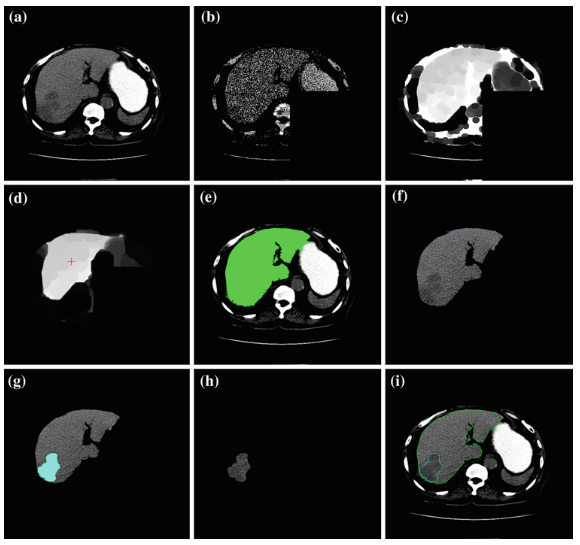
\includegraphics[width=0.7\linewidth]{images/Kumar2013_Fig5_v3}
	\caption{Liver segmentation pipeline after the placement of a seed at the estimated liver centroid position as detailed by \textbf{©Kumar et al. \cite{Kumar2013}}: (a) Original image, (b) simplified image, (c) eroded image, (d) cross indicates the centroid (seed point) on the eroded image, (e) region grown liver, (f) segmented liver after postprocessing, (g) AFCM clustered lesion, (h) segmented lesion, (i) segmented liver and lesion outlined in the original image}
	\label{Kumar2013_Fig5}
\end{figure}


Geometrical rules or local intensity properties often guide the growth
of the region. In Rusko et al. Susombooon et al., Kumar et al. the intensity in a given n-voxels-sized neighborhood is analyzed
to decide whether or not a point is added to the region \cite{Rusko2007, Susomboon2007, Kumar2013}. 
Phole and Toennies decided to iteratively test the homogeneity of the
region after adding candidate points \cite{Pohle2001}
. In Beck and Aurich, the filling step is controlled by a nonlinear
coupling criterion, which computes the weighted intensity difference
between a seed point and its neighborhood. Weights are controlled by a
non-normalized Gaussian function applied on both the distance to the
seed point and on intensity difference \cite{Beck2007}.\\
However region growing methods have the disadvantage to poorly handle
pathological livers, and often fail due to leakage in presence of weak
boundaries.


\subsection{Geometric deformable models}

Both geometric deformable models (aka active contours) and level set
based methods rely on boundary tracking to perform the segmentation.\\
The basic idea of \emph{active contours} (introduced in 1988) is to
come from an initial contour and deform it until it reaches the
contour of the object. The deformation function reaches its minimum when
the boundary of the object is found. The function used to deform the
contour is an energy function that tries to control the smoothness of
the curve and that is attracted by the object boundaries.\\
One of the main drawbacks of this method is that the final curve will
always have the same topology as the initial one, meaning for example
that multiple objects can not be detected. To overcome those limitations,
new models, based on the theory of curve evolution and geometric flows,
were designed.
Caselles et al. \cite{Caselles1997} proposed a formulation where finding the contour will be
equivalent to finding a geodesic curve of minimal weighted length, thus
the formulation of \emph{geodesic active contours} .\\
In the active contours formulation, a parametric characterization of the
boundary is utilized, whereas in the level set paradigm, they are
embedded as a time-dependent partial differential equation (PDE).
Osher and Fedkiw \cite{Osher2003} proposed a definition, where the boundary of an object
can be regarded as a zero-level set of a time-dependent function which
is evolving based on the speed at which the contour evolves along its
normal direction. The negative values correspond to voxels belonging to
the liver regions, and positive values to the outside. This paradigm was
first implemented by
Pan and Dawant \cite{Pan2001}, who used the level set technique for the automatic segmentation of liver
in CT scans. They realized that the classical formulation can not
accurately handle cases where weak boundaries are present in noisy or
non-uniform images. Therefore, they decided to use an accumulative
curvature-dependent speed function that would depend on the front past
history. In order to be compliant with abdominal CT scans segmentation,
a priori anatomical knowledge was added to the process by considering
the distance from the liver to the skin and the ribs. Initial detection
of the skin and the ribs is illustrated in the figure \ref{Pan2001_Fig5}.

\begin{figure}[ht!]
	\centering
	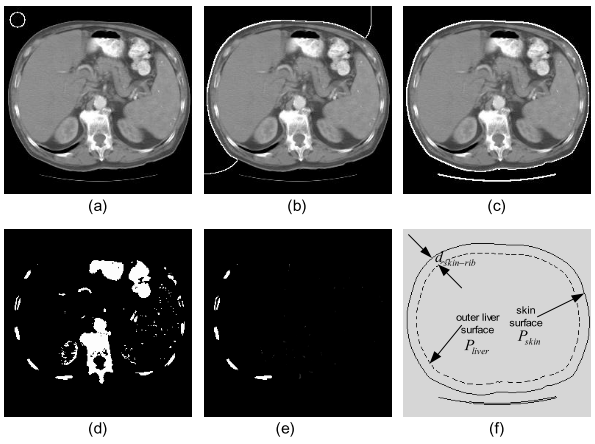
\includegraphics[width=0.7\linewidth]{images/Pan2001_Fig5}
	\caption{Skin surface localization (a-c) followed by the extraction of the ribs (d-f) as described by \textbf{©Pan et al. \cite{Pan2001}}}
	\label{Pan2001_Fig5}
\end{figure}


Wang et al. \cite{Wang2016} combined probabilistic atlas (PA) and level set to perform the segmentation of the liver. Training volumes were pre-processed before the liver region was
segmented, and stored with the denoised CT volumes. During the inference
phase, the different training denoised CT volumes are used to compute
the weighted PA for the current test patient. The liver ROI is then
extracted using the weighted PA, and improved by estimating 5 different
regions (heart, liver, right kidney, spleen and bone). Finally, a
combined shape-intensity model is generated from the training samples,
and used to refine the mask by level-set based segmentation.\\
Garamendi et al \cite{Garamendi2007}, proposed to segment the liver using a
geometric level set method. After manually placing a circle in the liver
region to segment, different candidates ROI were iteratively obtained by
computed gray-level properties inside and outside the given region, and
shifting the boundary by looking at local information around the border
pixels. This procedure is repeated until the border stabilizes.
Chi et al. \cite{Chi2007} proposed a segmentation technique based on active
contour. They placed the initial boundary by analyzing anatomical
properties of the patient such as the position of the rib cage, the
heart and the lungs. K-means clustering is added to reduce the variation
present in the candidate surface by detecting blood vessels, remaining
heart tissues, the liver, the kidney and the tumors. Finally, active
contour is used based on GVF (\emph{gradient vector flow}) combined with
a distance transform formulation which detects the liver boundary based on
the mask obtained for the previous slice .
Furukawa et al. \cite{Furukawa2007} combined rough segmentation based on MAP estimation and
level set method to achieve liver segmentation. To perform the rough
segmentation, the lungs are initially segmented and used to normalize
the different images. The liver as long as 3 other components
(right-kidney, heart and other tissues/organs or muscles) are segmented
using MAP with a PA as reference. Active contours are used to refine the
segmentation by re-using the definition provided by Catelles et al. and
adding a term based on the distance to the human body contours.\\ 
Lee et al. \cite{Lee2007} computed a speed image through a fast marching algorithm, by
looking at gradient magnitude in the original image. A rough
segmentation is retrieved by performing a 2.5D propagation after placing
seed points on the top and the bottom of the liver. A level set method
is implemented to refine the obtained area. The evolution of the
level-set based contour is controlled by the initial speed image values
and by the curvature. Vessels near the liver boundary can be added to
the final map using a rolling ball algorithm.
Wimmer et al. \cite{Wimmer2007} semi-automatically segmented the liver by extending 2D
cross-sectional annotations, in 3D using RBF and applied a level set
technique to refine the obtained volume. The initial area is obtained by
manually performing 2 cross-sectional segmentations per axis, and
extending them in 3D via RBF after sampling some points along the given
contours, as depicted in the figure \ref{Wimmer2007_Fig2}.
The level set reconstruction surface was then used to refine the
obtained shape. The function used takes into account the points
initially present after manual segmentation. This method however suffers
from errors when an initial surface includes high-contrast boundaries
not belonging to the liver, because they will tend to attract the
surface during the deformation process.


\begin{figure} [ht!]
	\centering
	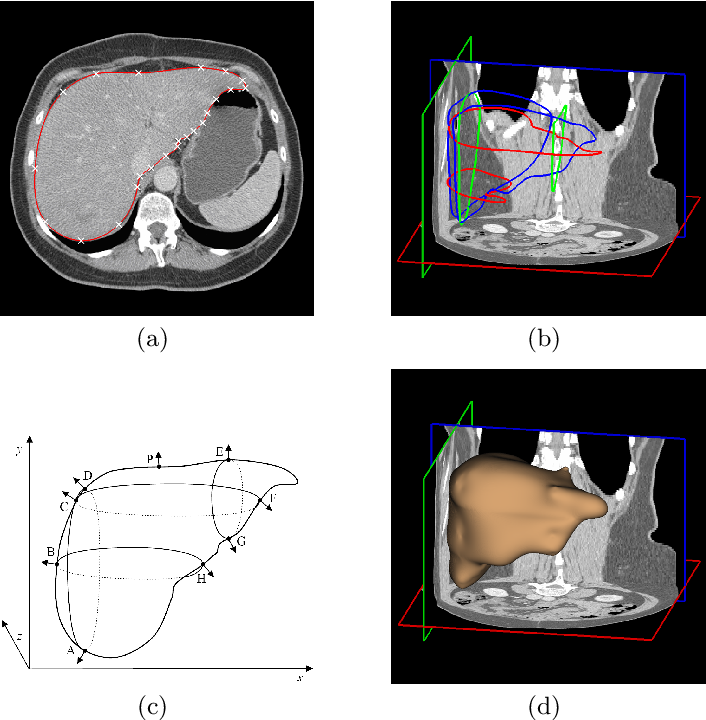
\includegraphics[width=0.5\linewidth]{images/Wimmer2007_Fig2}
	\caption{Semi automatic segmentation pipeline as proposed by \textbf{©Wimmer et al. \cite{Wimmer2007}}: (a) Manual delineation of a liver cross-section; spline control points are depicted in white (b) Six cross-sectional contours are defined, two for each orthogonal view orientation. (c) Visualization of calculated 3-D normals (d) Rendering of the interpolated surface.}
	\label{Wimmer2007_Fig2}
\end{figure}


Later, Wimmer et al. \cite{Wimmer2008} used an implicit active shape model to perform the
segmentation of the liver. To build the active shape model, one
segmentation is used as reference, and the rest of the training
segmentations are aligned to it. To convert the obtained masks into an
implicit representation, a signed distance map is computed for each mask
where grid points are assigned positive or negative Euclidean distance
to the boundary. The shape model is expressed based on the principal
component analysis of the signed distance maps. A level set function is
formulated based on the given shape model. To build the boundary, all
grid points in a narrow-band around the zero-level set are considered,
and their boundary profile is computed. A probability is assigned to
each point by considering the learned appearance model. Candidates
points are projected back to the zero level set, and the points with the
highest probability are kept. The obtained probability map is used in
GVF (\emph{Gradient Vector Flow}) to get the best contour.\\
Massoptier and Casciaro used a patch-based intensity approach to distinguish
hepatic tissues from other abdominal organs, and refine the obtained
boundary by implementing active contour with GVF. The liver segmentation
was followed by a liver lesions segmentation via k-means clustering \cite{Massoptier2008}. Wimmer et al. \cite{Wimmer2009} built later a shape model based on nonparametric density
estimates. The appearance model is obtained by computing profiles for
points in a narrow band along the zero-level set boundary. To evaluate
the boundary probability for the points present in the narrow-band, they
used a kNN classifier. A region model built upon a cascade of
classifiers is implemented to complete the boundary model, and prevent
it to stop at local extremum. Finally, a shape model based on Parzen
density estimation constrains the level set evolution. Song et al. \cite{Song2009} pre-segmented the liver using an edge detector, and
refined the segmentation with a curvature-based level set algorithm .
Three B-splines surface models are built knowing the position of the
lung, and assuming that the bottom of the liver corresponds to the
bottom of the left lobe. Those three surface models are implemented in a
graph-based optimal surface fitting scheme to remove possible false
positives and the remaining part is used as initialization for the level
set evolution.\\
Suzuki et al. \cite{Suzuki2010} preprocessed the image via anisotropic diffusion
filtering to reduce the noise on the CT images, and combined it with a
scale-specific gradient magnitude filter to enhance the liver
boundaries. The obtained image is handled by experts to put seed points
for the fast marching level-set algorithm. Next to the boundary
estimation, the geodesic active contour level set segmentation refined
the initial contour. Their technique uses the gradient-enhanced image as
a speed function, so that the front expansion speed slows down in
regions having high gradient and accelerates where the gradient is low.
The different steps of their method is depicted in the figure \ref{Suzuki2010_Fig3}.

\begin{figure}[ht!]
	\centering
	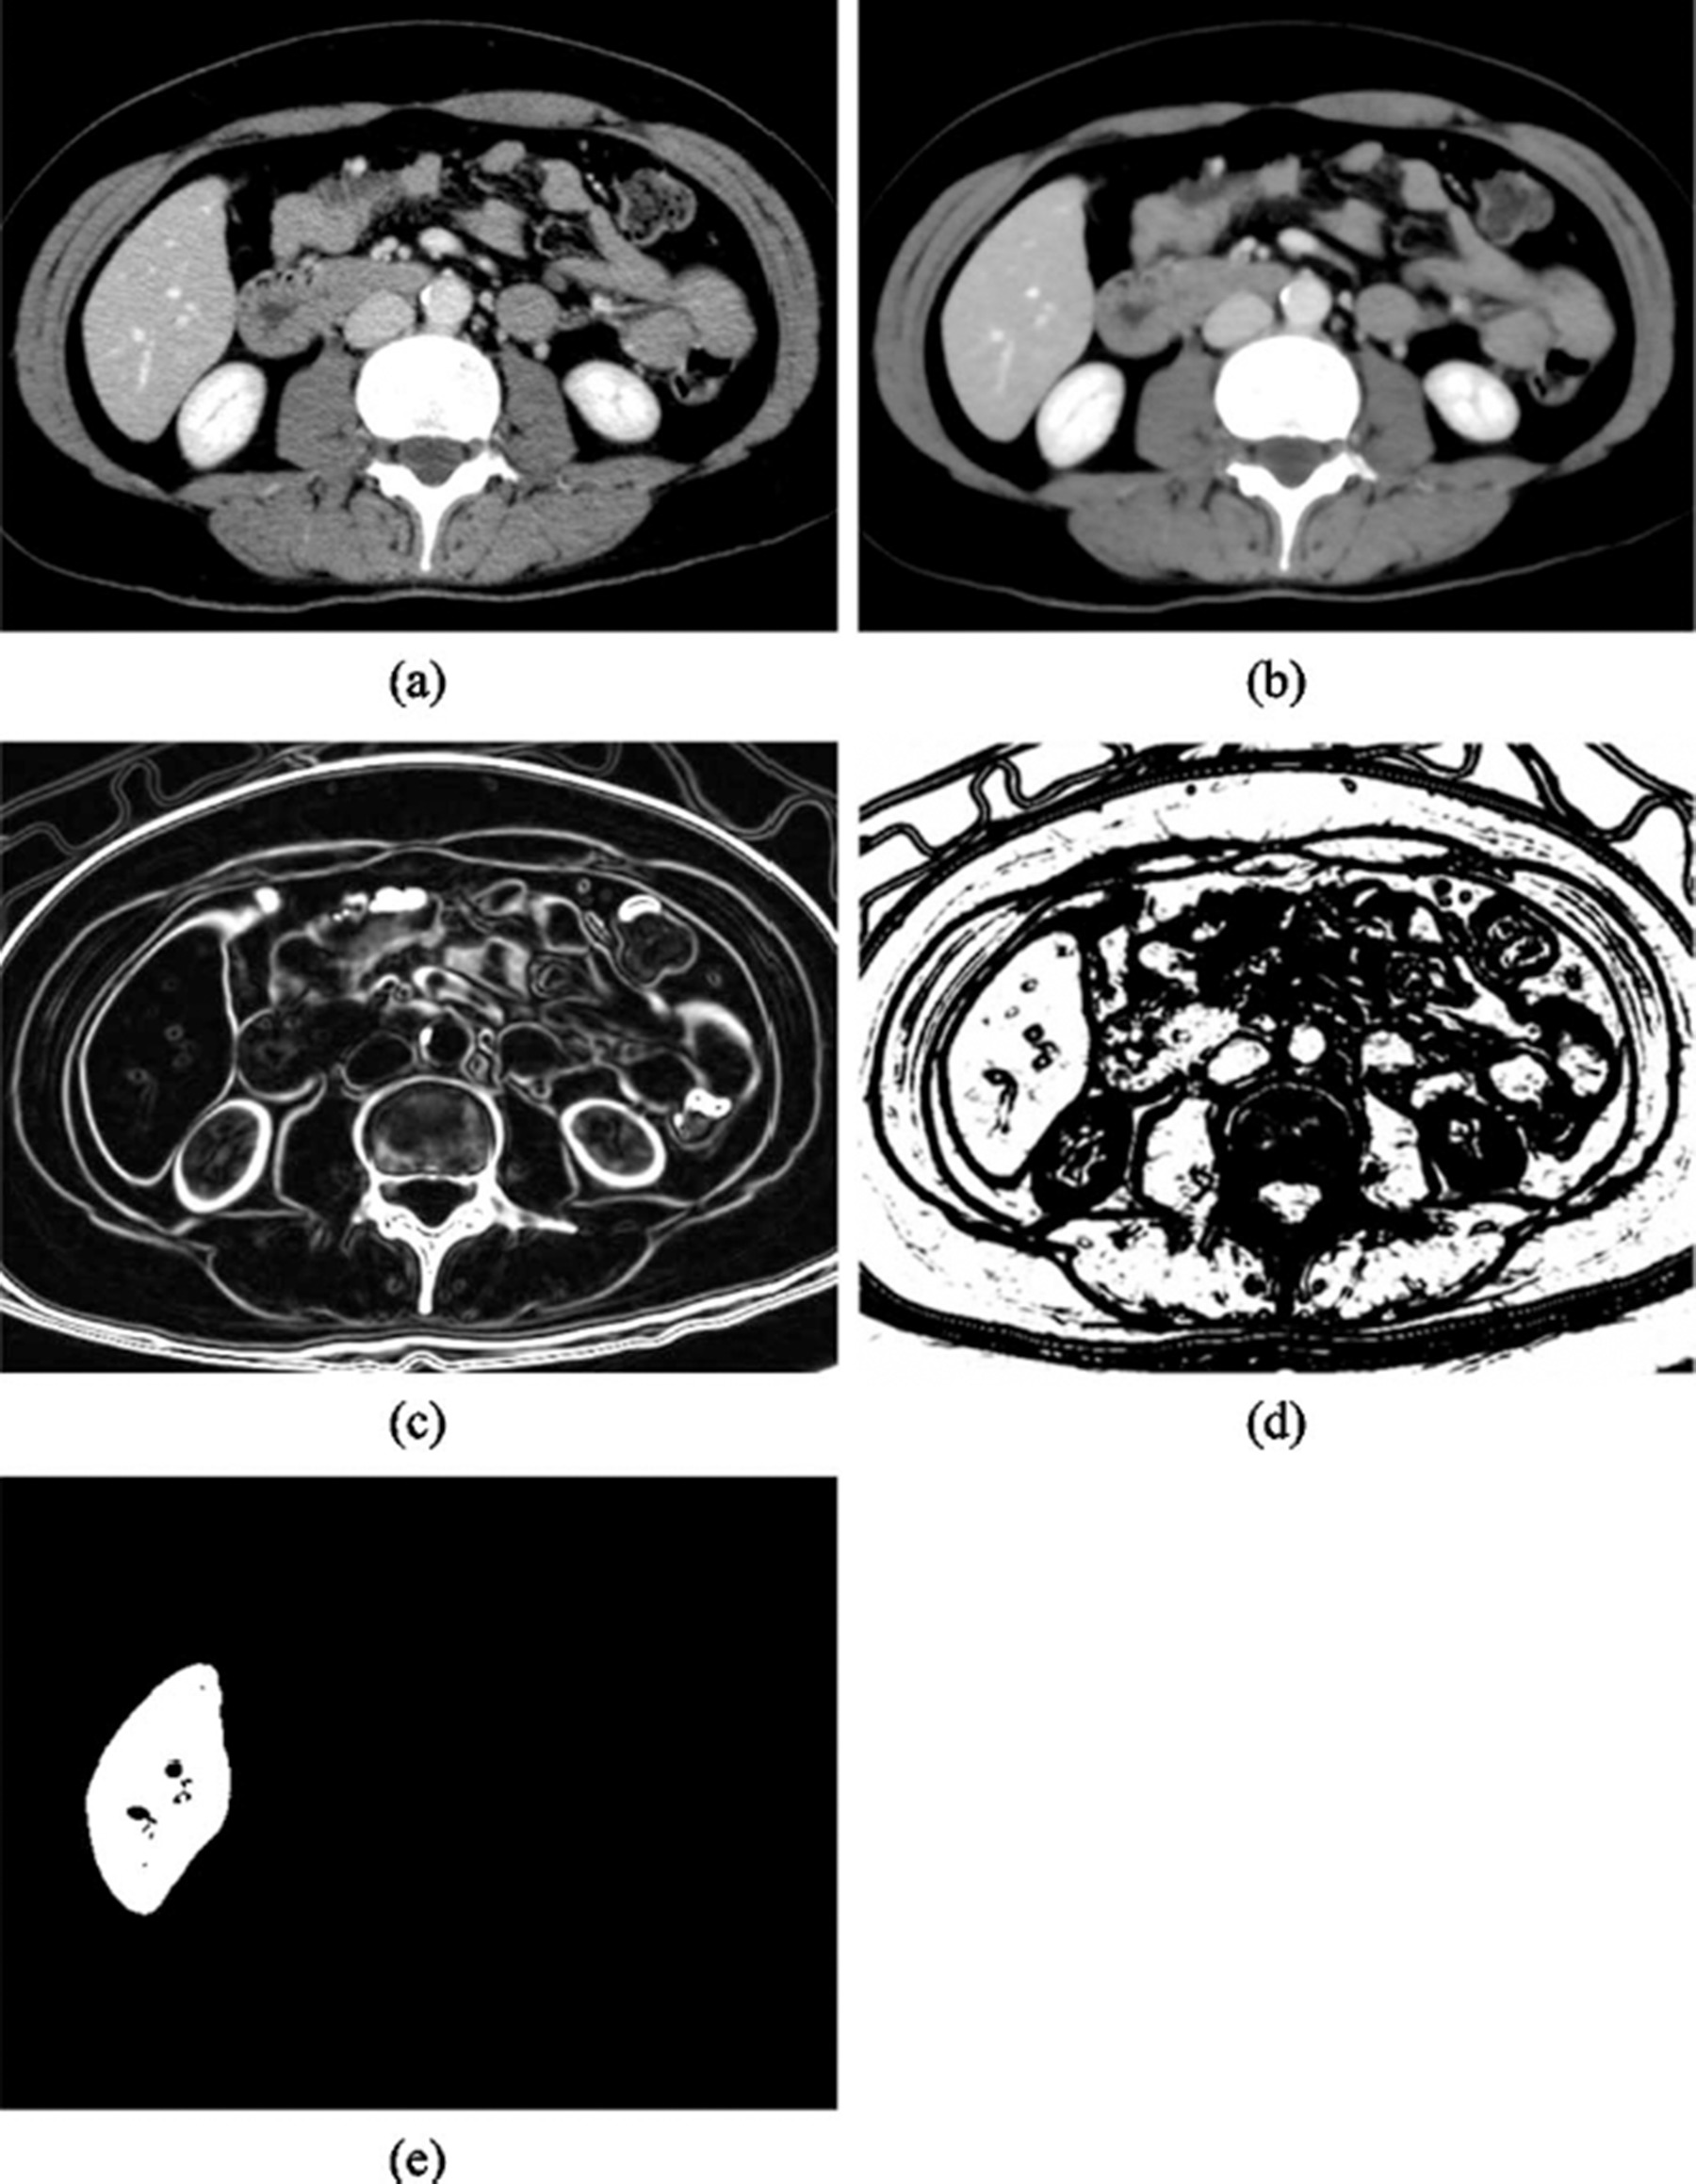
\includegraphics[width=0.5\linewidth]{images/Suzuki2010_Fig3}
	\caption{The different steps of the segmentation process developed by \textbf{©Suzuki et al. \cite{Suzuki2010}}: (a) Original CT image. (b) Anisotropic diffusion noise reduction. (c) Scale-specific gradient magnitude calculation. (d) Nonlinear grayscale conversion. (e) Geodesic active contour segmentation.}
	\label{Suzuki2010_Fig3}
\end{figure}


To segment the liver, Platero et al. \cite{Platero2011} first aligned the different training shapes, and captured
their variability via principal components analysis when building the
level set function. The narrow-band technique is used to select boundary
candidates whose profiles are computed. Their method, incorporating
shape based priors as long as edge and region-based knowledge is then
implemented.
Jimenez et al. \cite{Jimenez-Carretero2011} proposed an optimized level set where the parameters are
defined at each stage by means of multi-curvature, and where the liver
segmentation is iteratively corrected in a pyramidal process. A fine
details strategy tries to prevent problems that can come from the use of
a narrow-band technique when searching for the boundary, by removing
outlier pixels. An additional step is semi-automatically used to impose
local curvature constraints.

Algorithms based on active contours were historically considered as one
of the most utilized segmentation methods \cite{Moghbel2018}. Later after the introduction
of active-contours and level set, a new algorithm called Graph Cut
segmentation was introduced by Boykov et al. to propose an alternative to boundary-based approaches \cite{Boykov2001}.

\subsection{Graph-theory based methods}

The random walker algorithm, which was introduced by Grady et al. \cite{Grady2006} and the Graph Cut (GC) method correspond to
semi-automatic\footnote{can be fully automatic in some cases} methods where the user provides seeds for both the
background and the region to segment. They both interpret pixels of the
image as nodes on a graph where edges represent adjacency between
pixels. The weights on the edges correspond to the similarity between
adjacent pixels \footnote{The random walker will compute, 
for each unlabeled pixel, the highest probability 
that a random walker reaches the first labeled pixel 
whereas the GC will try to find the optimal cut for the entire image 
considering all the labeled seed, thus being more likely 
to fail in case of weak boundaries \cite{Grady2006}}.

The GC will then try to find the minimum cost function between all
possible cuts on the graph to separate the object from its background.

GC often suffers from the ``small cut'' problem where only the seeds are
separated from the rest of the image, whereas the random walker method
does not suffer from this problem since it is not aiming for the
smallest boundary, as represented in the figure \ref{Grady2006_Fig5}.

\begin{figure}[th!]
	\centering
	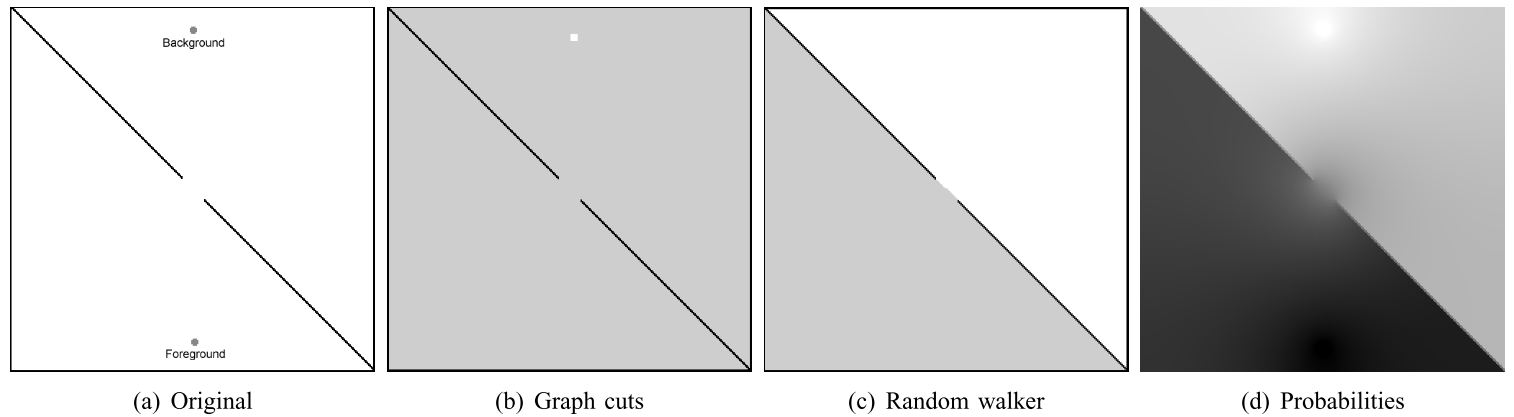
\includegraphics[width=0.8\linewidth]{images/Grady2005_Fig5_v3}
	\caption{Comparison of random walker algorithm to graph cuts for a weak boundary with small seeds. Note that a 4-connected graph was used in these experiments. (a) Original (synthetic) image created with a diagonal black line with a section completely erased. (b) Graph cuts solution Since surface area of seeds is smaller than the weak boundary, the smallest cut minimally surrounds the seeds. (c) Random walker solution. (d) Probabilities associated with the random walker algorithm offer a notion of segmentation confidence at each pixel. \textbf{©Grady et al. \cite{Grady2006}}}
	\label{Grady2006_Fig5}
\end{figure}


%The region growing method is based on the selection
%of a seed pixel and the neighboring pixels with similar statisti-
%cal values come together to become a region. It uses standard
%deviation and average intensity to grow the area [7]. The most
%commonly used procedure of changing the seed points in region
%growing method is (1).

%In this method, the image is modeled as graph. The nodes
%represent the pixels in the image and pixels are linked to the
%other nodes by the weighted edges according to the similarity
%to the neighboring pixels. The interactive image segmentation
%method requires from the user to indicate seed points as starting
%points. These seed points are usually divided into two classes
%as the background and the foreground, and seed points which
%belong to more classes can also be indicated. For this method,
%seeds are selected from the experimentally determined interval
%as region growing method. User defined seed points are called
%as labelled pixels. The other pixels in the image are called as
%unlabeled pixels and an imaginary random walker continue to
%process from these unlabeled pixels. This walker moves to the
%other pixels depending on the edge weight. The probability of
%the first arrival to these pixels is calculated along the random
%walk for all labelled pixels. The first labelled seed which has
%the highest probability of random walk leaving from an unla-
%beled pixel, is labeled with the same label value according to
%the calculated probabilities. According to this method, after all
%the unlabeled pixels are labeled, image is segmented into parti-
%tions.


The random walker algorithm has been implemented by Maier et al. \cite{Maier2008} to proceed the segmentation of the liver. Seed points were
automatically detected in several regions in a slice-wise fashion. Based
on the skin surface and some anatomical assumptions, the rib cage and
liver seed points are generated. Background seeds are obtained by
detecting the air, the fat and the bones.
Dong et al. \cite{Dong2016} proposed a random walker implementation where adjacent slices are
considered as prior knowledge when segmenting the liver and the spleen in the current slice. Two
slices are chosen so that they present the largest cross sectional area
of both the liver and the spleen. Seeds are manually placed on these
slices and updated on adjacent slices via GMM (\emph{Gaussian Mixture
	Model}) and intensity constraints through \emph{Narrow Band
	Thresholding} (NBT), before the modified random walker segment the organs in a
slice-wise fashion. Details of the execution can be found in the figure
\ref{Dong2016_Fig3}.

\begin{figure}[th!]
	\centering
	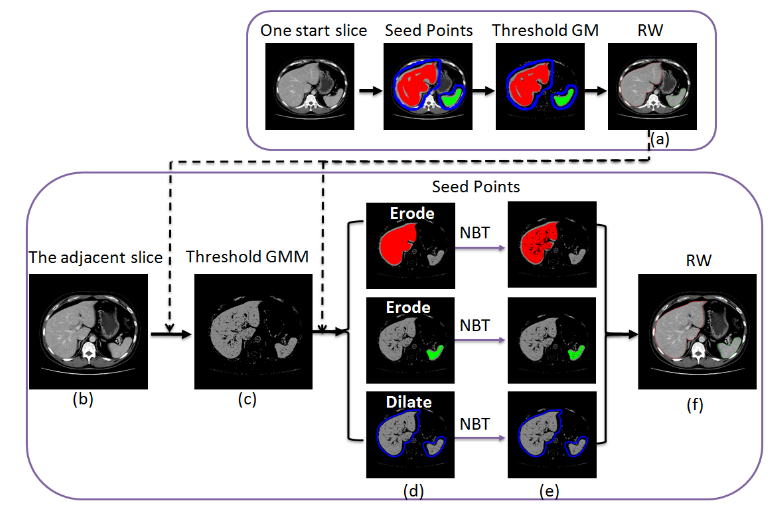
\includegraphics[width=0.7\linewidth]{images/Dong2016_Fig3_v2}
	\caption{Segmentation Pipeline detailed by \textbf{©Dong et al. \cite{Dong2016}}: (a) The segmented liver (red) and spleen (green) of the previous slice; (b) The current slice; (c) Candidate pixel by applying a threshold to the GMM; (d) The rough objects (red and green) and background (blue) seed points; (e) The fine seed points using the NBT method; (f) The segmentation results}
	\label{Dong2016_Fig3}
\end{figure}


Beichel et al. \cite{Beichel2004} used a graph-cut method to propose an initial liver
region which can interactively be segmented by the users. The cost of
the graph cut segmentation is specified by taking region and boundary
properties into account. The region term evaluates the gray-level
similarity in the neighborhood of a given point and compares it to the
intensity of the seed points. The boundary term is computed from the
local gradient information.
Massoptier and Casciaro \cite{Massoptier2007}, introduced a GC method initialized by an adaptive
threshold to perform the liver segmentation. The thresholding was implemented by detecting the most likely
liver intensity based on patch partition of the abdominal slices. The
energy function took both a region and a boundary-based term into
account.
Shimizu et al. \cite{Shimizu2011} combined a statistical atlas-based approach and a graph
cuts algorithm to segment the liver. The graph supports an energy
function including a local term, a boundary term and a shape-based term
computed from the gradient of the initial region.\\
The key part of graph cut methods is to define a relevant energy
function, which can sometimes be difficult.\\
Probabilistic atlases (PA) and Statistical Shape Models (SSM) both
utilize prior information on the liver. The main goal of those
techniques is to improve the segmentation by not relying only on the
gray-level distribution since it was proven not to be sufficient,
especially knowing the intensity similarity that the liver presents with
close organs \cite{Zhou2006, Park2003, Slagmolen2007, Rikxoort2007}.

\subsection{Probabilistic Atlases}

To construct a probabilistic atlas, images from the training set are
registered to a reference image, whereas manual delineations are warped
onto the template image and averaged to get a probability of belonging to the liver for each voxel of the space. The generated atlas is then
incorporated in the segmentation process. The studies differ one another
on the way they construct the atlas, and on how it is incorporated in
the segmentation process. 
Park et al. \cite{Park2003} used the MIAMI method (\emph{Mutual Information for Automatic
	Multimodality Image Fusion}) which combines a TPS-based (\emph{Thin
	Plate Splines}) registration method with MI (\emph{Mutual Information})
as a similarity metric to segment multiple abdominal organs. The TPS is a registration method that uses
control points as constraints to the interpolating function. They used
36 control points that were placed in different organs by experts, and
they performed the registration separately for each organ to not be
biased by the presence of more control points on the liver surface. The
different points can be seen in the figure \ref{Park2003_Fig1}.

\begin{figure}
	\centering
	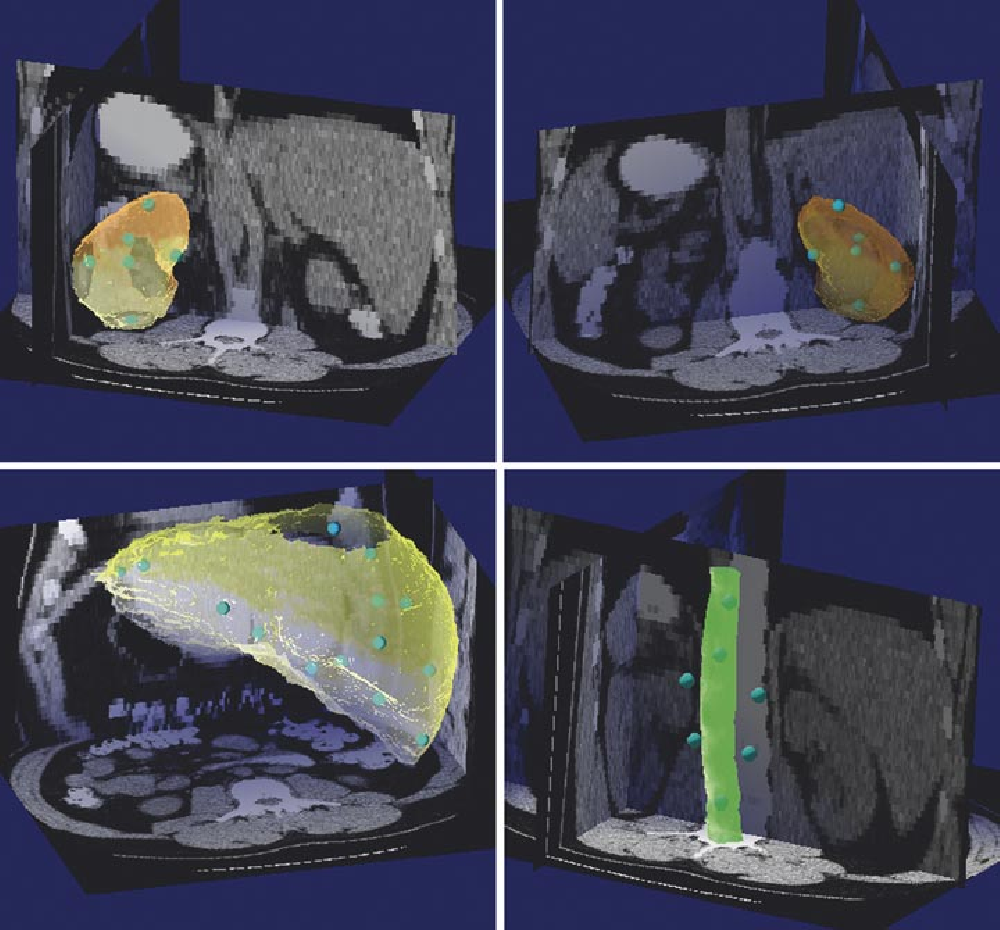
\includegraphics[width=0.5\linewidth]{images/Park2003_Fig1}
	\caption{Example of control points distribution used in the MIAMI method as described by \textbf{©Park et al. \cite{Park2003}}}
	\label{Park2003_Fig1}
\end{figure}


Zhou et al. \cite{Zhou2006} extracted the so-called ``anatomical structure'' of each
patient, which is composed of the bone structure (determined using
gray-level thresholding) and the diaphragm (based on the shape of the
air within the lungs) to obtain the liver segmentation. A matrix transformation of the TPS is calculated
between each one of the training cases and a predefined standard
anatomical structure \cite{Zhou2005}.
The atlas is then computed by combining the obtained positions using a
voting strategy. When performing the segmentation, the same strategy is
performed: the current patient's anatomical structure is estimated, and
deformed to the standard one. The gray-level distribution is also used
to compute the final probability as well as the spatial location as
depicted in the figure \ref{Zhou2006_Fig4}.
\begin{figure}[th!]
	\centering
	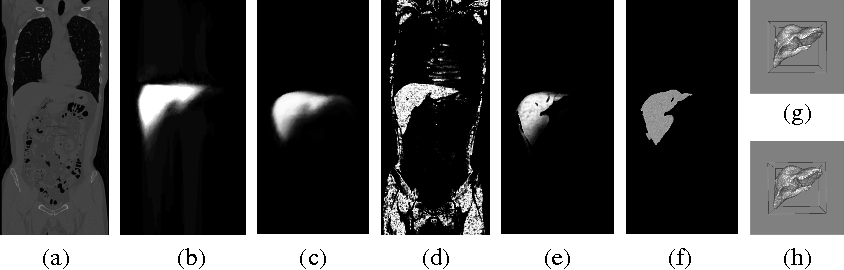
\includegraphics[width=0.9\linewidth]{images/Zhou2006_Fig4}
	\caption{Example of liver segmentation with the different slices results as described by \textbf{Zhou et al. \cite{Zhou2006}}: (a) original CT image (1 coronal slice), (b) liver atlas, (c) P(B) : liver probability on spatial location, (d) P(C|B) : liver probability on density, (e) P(A) : liver probability, (f) liver segmentation result (1 coronal slice), (g) ground truth of liver (3-D view), (h) liver segmentation result (3-D view)}
	\label{Zhou2006_Fig4}
\end{figure}

Slagmolen et al. \cite{Slagmolen2007} resampled all training images to a selected one using
affine registration with MI as the similarity metric, followed by a
non-rigid registration guided by a surface distance metric when segmenting the liver. A mean
morphology is defined by averaging, for each patient in the training
set, its deformation field to every other image. Each patient is then
deformed using its corresponding mean deformation field. And finally the
obtained images are averaged on their intensities to obtain the atlas.
Van Rikxoort et al. \cite{Rikxoort2007} decided to first find the vertical range that most likely
contains the liver by looking at HU values covering the lungs and
extract slices above them. They trained a kNN classifier with both gray
level features (obtained from both the gradient computation and the
Gaussian derivatives at various scales), positional features through the
coordinates in the liver space, and an additional feature obtained by
computing the proportion of the liver above, behind and to the left of a
given voxel. No concrete atlas was created here, but the current test
volume is registered to each training sample in a \emph{non-rigid
	multi-atlas segmentation}, before applying the classification to refine
the obtained region.
Li et al. \cite{Li2010} constructed a liver and a rib-cage probabilistic atlas . Both
atlases were built iteratively to reduce the dependence to the reference
patient, before a liver segmentation is obtained. 
Linguraru et al. \cite{Linguraru2009} created the atlas by normalizing the liver coordinates of
each patient relative to the xiphoid, and used those coordinates in the
size-preserving affine registration process, by randomly selecting a
patient as reference.

In those different studies, the segmentation method applied is often
related to the way the atlas is created. Therefore Park et al. decided to complete the segmentation step by incorporating the
atlas information in a bayesian framework which combines MAP and EM,
with gray level distribution as basis \cite{Park2003}. The segmentation is then refined
using a MRF (\emph{Markov Random Field}) regularization step. In the
other studies, non-rigid or elastic registration is performed from the
atlas to the target case \cite{Slagmolen2007, Linguraru2009, Li2010}, after constraining the input, using either manually defined
ROI around the liver \cite{Slagmolen2007}, or analyzing the gaussian intensity distribution to
remove irrelevant parts \cite{Li2010}.

\subsection{Statistical Shape Models}

Statistical shape models on the other hand try to extract features of
the model instead of building an average map.

They were first described by Cootes et al. \cite{Cootes1995}, 
who introduced the concept of Active Shape Models (ASM) which
are built from a set of segmented training images and consist of two
parts, a geometrical model, and a local appearance model. The
geometrical model describes the shape and is represented by a PDM
(\emph{Point Distribution Model}), a dense collection of landmark points
on the surface of the object. Given the location of the landmarks for
each training case, a principal component model can be built in order to
approximate all valid shapes. The local appearance model describing the
boundary, is used as an additional one to detect the modeled shape in
the new image. It is based on the local gray value appearance around the
boundary. A PCA or a kNN model can be used to determine the possible
profiles at each landmark. The model is then guided by internal
forces that should keep the shape of the deformable model similar to the
one of the underlying SSM, and external forces that drive the deformable
surface towards the best fit to the data.

To perform the segmentation of the liver, Montagnat and Delingette \cite{Montagnat1997} followed 
this scheme by deforming the model with
global constraints (shape constraints and transformation constraints) to
reduce the degrees of freedom, and registered the obtained model on the
volumetric data including an additional external force based on local
gradient computation.
Lamecker et al. \cite{Lamecker2004} proposed a model that combined global constraints that
minimized the geometric distortion for shape correspondence, and local
constraints by considering the intensity profiles for the boundary
search. The evolution of the boundary search for one example can be seen in the figure \ref{Lamecker2004_Fig9}.

\begin{figure}[ht!]
	\centering
	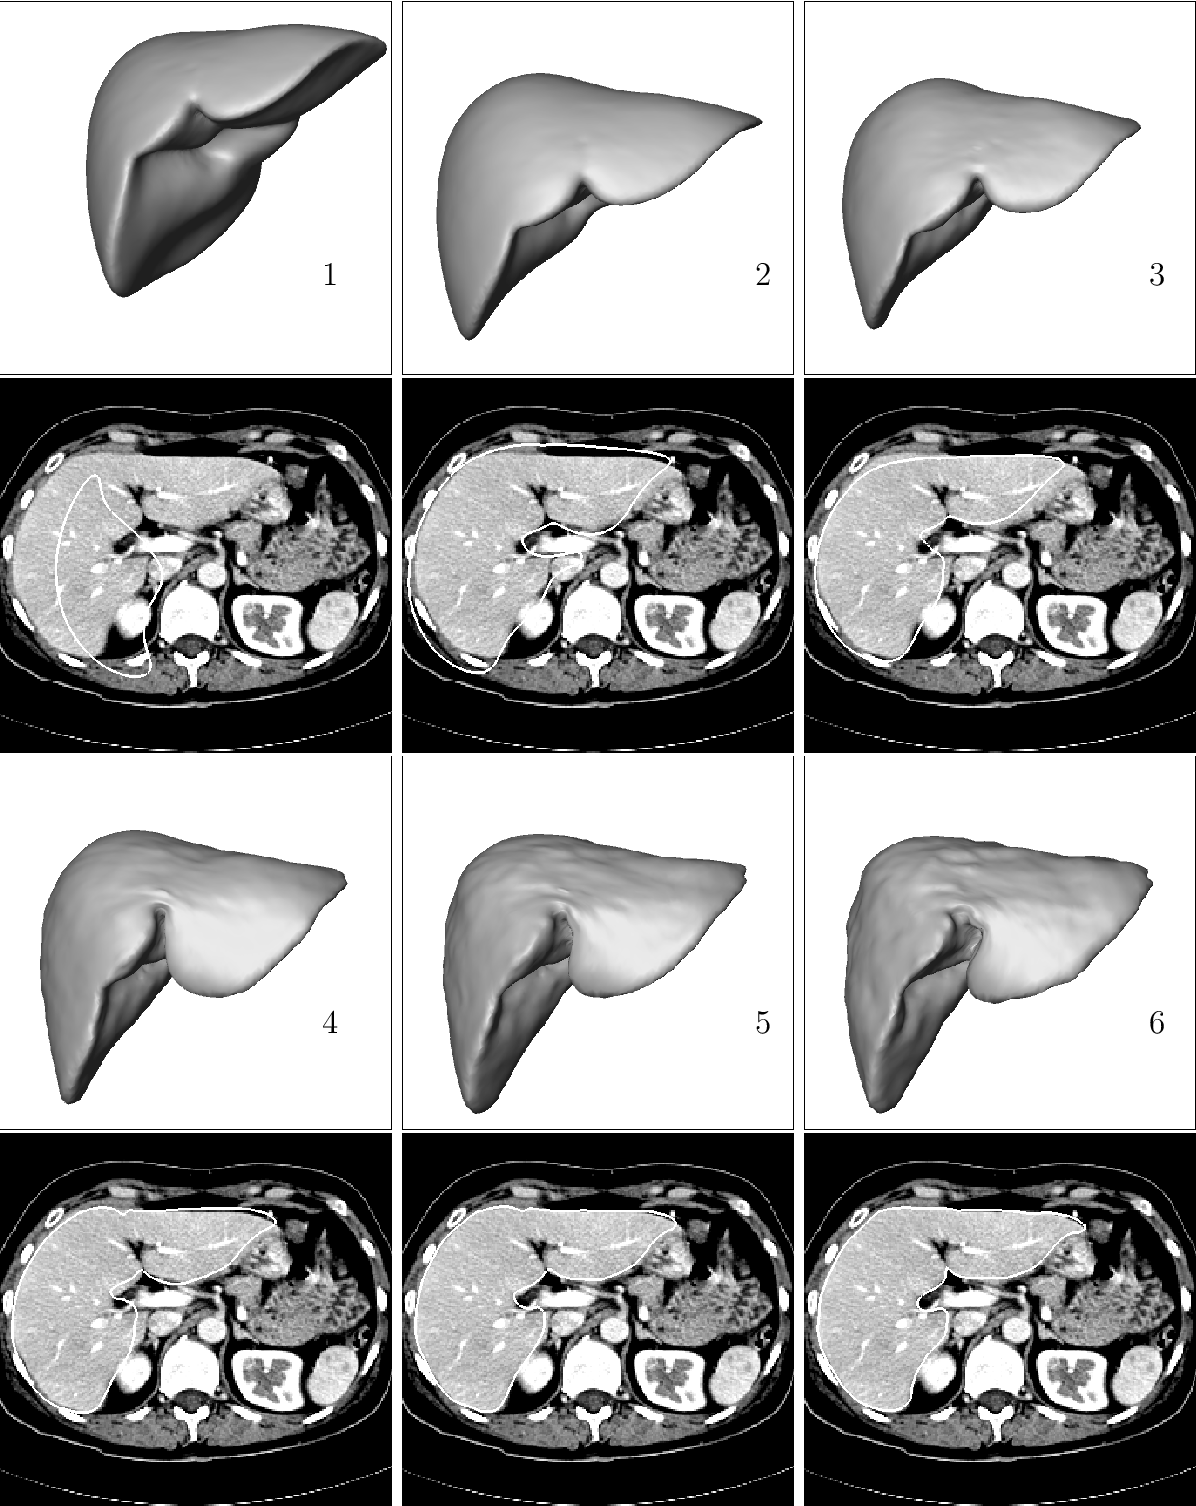
\includegraphics[width=0.6\linewidth]{images/Lamecker2004_Fig9}
	\caption{Evolution of boundary search in one example as described in \textbf{©Lamecker et al. \cite{Lamecker2004}}: At each of the six steps the model at its current position and shape is shown as a 3D surface. Below each surface one axial slice with the intersection line of the surface is displayed. Step 1: initial positioning of the mean model in the CT data such that the upper borders of the bounding boxes match. Step 2: result of the initial optimization of the position parameters. Step 3-5: results of the combined position and shape optimization with increasing number of shape modes (3, 9, 21). Step 6: final result (42 shape modes)}
	\label{Lamecker2004_Fig9}
\end{figure}


Heimann et al. \cite{Heimann2007} used an evolutionary algorithm to create a population of
possible liver shape configurations and evaluated all the population members
using a local appearance model based on a kNN-classifier utilizing the
profiles.  Saddi et al. \cite{Saddi2007} constrained the boundary of the liver to fit the
global-shape learned from the training samples, and refined it locally
using a template-matching algorithm. For both problems, they used the
intensity distribution inside and outside the liver to find the best
region to segment. Zhang et al. \cite{Zhang2010} performed the detection of the liver using a 3-D
generalized Hough transform so that each vertex on the surface of the
average shape model is stored in a table, by considering its coordinates
relative to the liver centroid. The most probable liver centroid is
computed for a given test image. A search is then performed to determine
the points belonging to the boundary knowing the intensity distribution
inside the liver and the properties of the gradient along the boundary.
An optimal surface detection algorithm is finally applied to refine the
obtained boundary by using a graph-search strategy. The different steps
of the algorithm can be visualized in the figure \ref{Zhang2010_Fig5}.

\begin{figure}[th!]
	\centering
	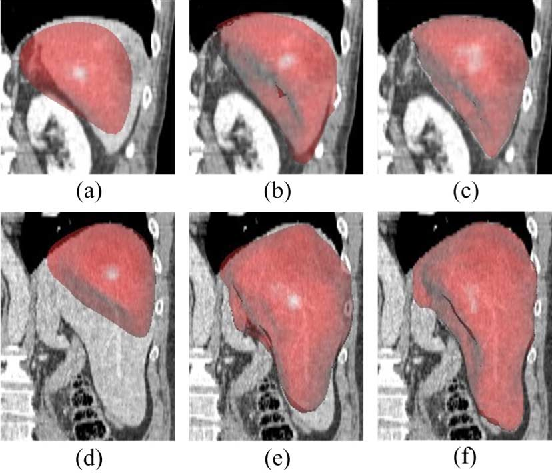
\includegraphics[width=0.5\linewidth]{images/Zhang2010_fig5}
	\caption{State of the surface mesh in a coronal slice from back after each segmentation step. The top row shows a relatively easy case while the bottom row shows a relatively difficult case. (a) and (d) After localization by 3-D GHT. (b) and (e) After model subspace initialization. (c) and (f) Final result after optimal surface detection. \textbf{©Zhang et al. \cite{Zhang2010}}}
	\label{Zhang2010_Fig5}
\end{figure}


Ling et al. \cite{Ling2008} went further by proposing a hierarchical segmentation of
the liver in a coarse-to-fine fashion. For the training process, a
hierarchical shape model is obtained by downsampling the resolution of
an initially obtained dense mesh. Each layer of the pyramid then
contained the mean shape as long as the different modes that capture
shape variations for the given resolution. During the inference, the
pose estimation is performed using a MSL-based  approach (\emph{Marginal Space Learning}) to reduce the
dimensionality of the research \cite{Zheng2007}. The model is then upsampled to the
finest resolution using local boundary refinement. At the finest
resolution, a patch-based approach is implemented to refine the obtained
boundary.
Seghers et al. \cite{Seghers2007} used multiple local shape models instead of a global one to segment the liver.
A grid search is used for the landmarks candidates detection, then, an
intensity model selects the best landmarks in a given test image by
analyzing the intensity profiles. This search is performed in a
multi-resolution manner by changing the size of the grid. A shape model
was built at each edge of the geometrical model, where an edge is
connecting two landmarks.
Erdt et al. \cite{Erdt2010} tried to determine the regions where high deformations
are expected by looking at the curvature. They first built the model
based on the data present in the training set, and then constrained it
locally using the curvature and the gradient at each landmark point.
Examples of how the incorporation of local curvature can improve the liver
segmentation results are depicted in the figure \ref{Erdt2010_Fig3}.

\begin{figure}[th!]
	\centering
	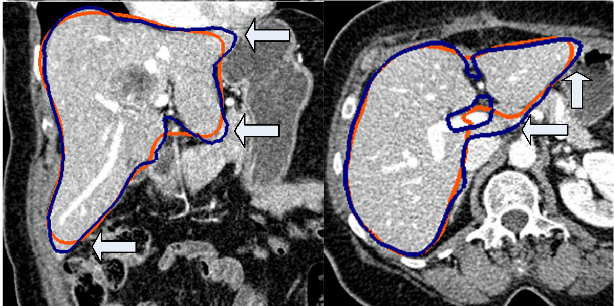
\includegraphics[width=0.4\linewidth]{images/Erdt2010_Fig3}
	\caption{Example of how the incorporation of the curvature improved the quality of the segmentation as reported by \textbf{©Erdt et al. \cite{Erdt2010}}}
	\label{Erdt2010_Fig3}
\end{figure}


A common drawback of SSMs is their lack of flexibility. To combat this
limitation, some studies combined the SSM with a free form deformation
step to achieve better performances. For example, Kainmüller et al. \cite{Kainmueller2007} built a SSM based on a PCA analysis of the given shapes
present in the training dataset, and to add flexibility to the model, a
free-form deformation step based on the computation of 3-vector fields
was conducted. During the deformation, they considered the general
intensity distribution of the liver, the local displacements and they
also tried to preserve the shape features of the initial model.\\
Okada et al. \cite{Okada2008} combined both PA and SSM in their study to segment the liver. The PA was
constructed from the different training cases by first registering the
volumes to a standardized patient space using non-rigid registration of
the abdominal cavity. The registration target was defined by experts
describing the standard position and shape of the liver. The atlas was
then computed by averaging the binary registered liver masks. The
multilevel shape model (ML-SSM) is obtained by dividing the liver shape
recursively into patches, and performing a PCA for each one of them. An
example of construction of ML-SSM can be seen in the figure \ref{Okada2008_Fig1}.
For each test case, the atlas was combined with the gray-level
distribution of the patient to obtain an initial liver region. A shape
model was then built from this area and the ML-SSM is employed to
segment the different patches, by adding an adhesive constraint to
eliminate inconsistencies between adjacent patches. They later improved
the efficiency of their method by constructing the PA hierarchically,
where the different structures are constrained by the shape of the organ
in the next highest hierarchy level. Three levels were handled, the
abdominal cavity, the liver, and finally both the vena cava \& the
gallbladder. They extended the ML-SSM to an organ-based relationship and
defined the MO-SSM (Multi-Organ SSM) \cite{Okada2008}. The MO-SSM is constructed by combining ML-SSM for the
different organs of interest. As a result they improved the accuracy in
the regions concerned by the MO-SSM.

\begin{figure}[th!]
	\centering
	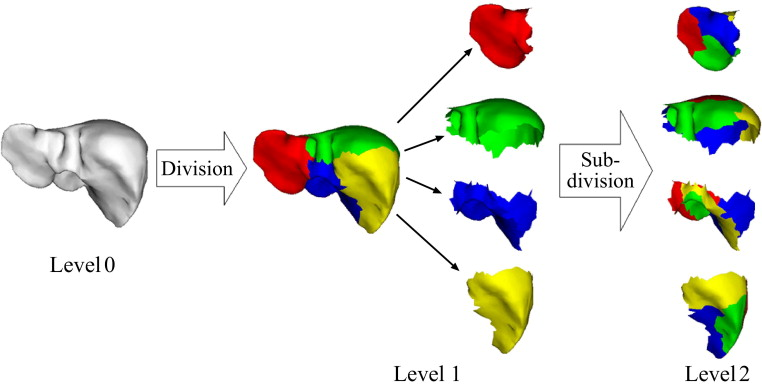
\includegraphics[width=0.7\linewidth]{images/Okada2008_Fig1}
	\caption{ Hierarchical division of the liver shape for multi-level statistical shape model as described by \textbf{©Okada et al. \cite{Okada2008}}}
	\label{Okada2008_Fig1}
\end{figure}


Apart from the lack of flexibility, SSMs suffer from a low number of
training samples, and also hardly deal with low contrast between the
liver and its surrounding or within the liver directly \cite{Saddi2007, Lamecker2004}. Examples of those limitations are depicted in the figure \ref{Saddi2007_Fig}.

\begin{figure}[th!]
	\centering
	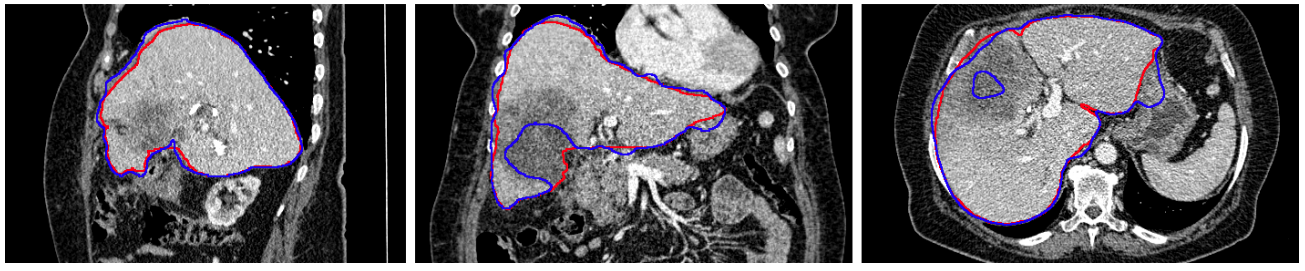
\includegraphics[width=0.7\linewidth]{images/image21}
	\caption{Example of errors obtained during the segmentation process as exposed by \textbf{©Saddi et al. \cite{Saddi2007}}}
	\label{Saddi2007_Fig}
\end{figure}

\subsection{Methods integrating machine learning based steps}

Some studies decided to combine the aforementioned techniques with the introduction of
machine learning methods such as shallow neural networks or SVM
(\emph{Support Vector Machine}) to segment the liver and potentially its tumor.\\
Tsai and Tanashi \cite{Tsai1994} used a neural network based on regional histogram to get
a rough liver segmentation. Several post-processing steps were added,
such as Laplacian filtering to obtain the boundary followed by a
smoothing using B-spline functions.
Gao et al. \cite{Gao1996} first located the liver by extracting peaks on gray-level
histograms, and applied domain-based knowledge to remove irrelevant
tissues. The liver region is refined based on adjacent slices
properties, before a boundary refinement is performed via a deformable
contour technique.
Schimdt et al. \cite{Schmidt2007} incorporated a set of intensity distributions,
neighboring relationship between organs and geometrical constraints to
segment different parts of the abdomen. Their study was based on several
anatomical assumptions, but fails when the liver presents a slightly
non-standardized aspect, especially when large tumors are present.
Freiman et al. \cite{Freiman2008} applied a multi-resolution, multi-class smoothed Bayesian
classification followed by morphological adjustments and an active
contour refinement for the segmentation of the liver. The classification
was performed by iteratively looking at liver and potential tumor
gray-level distributions. MAP rule is applied for the two classes. The
liver region is adjusted using morphological operations, before an
active contour refinement step based on gray-level intensity gives the
final segmentation.
Freiman et al. \cite{Freiman2011} further proposed a method for the semi-automatic segmentation of
liver tumors, where a SVM classification is employed to separate healthy
and tumorous tissues. A 3D energy function is then applied using
affinity constraints to get the final VOI.
Florin et al. \cite{Florin2007} proposed a shape model to segment the liver, that will describe the shape
variations only using a small number of key slices. This model, called Sparse Information Model, consists of key slices that are selected to be
sufficient so when combined with an interpolation function, the 3D
volume can be reconstructed. Those key slices are further used for the
segmentation but the result is highly sensitive to initializations.\\
To segment the liver, Schenk et al. \cite{Schenk2000} combined the ``livewire'' algorithm, which is a semi-automatic 2D segmentation method, with a
shape-base model to approximate the contour between the manually defined
slices. The interpolation used to combine the user-defined segmentations
is an object-based interpolation considering the distance transforms.
Maklad et al. \cite{Maklad2013} proposed to segment the liver by analyzing the blood vessels
structure. Abdominal blood vessels are first enhanced via bias field correction as depicted in the figure \ref{Maklad2013_Fig1}, and then extracted through thresholding
and region growing techniques. Those vessels are further classified into
hepatic and non-hepatic ones by applying distance transforms. The
boundary between the liver and its surrounding organs is then
constructed equidistantly from the hepatic vessels and the non-hepatic
ones. A post-processing step is finally applied to refine the obtained
area, by filling holes and classifying boundary tumors as belonging or
not to the liver based on their relation to hepatic blood vessels.

\begin{figure}[th!]
	\centering
	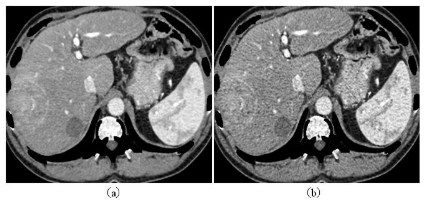
\includegraphics[width=0.5\linewidth]{images/Maklad2013_Fig1}
	\caption{Results of the blood vessels enhancement: (a) before enhancement (b) after enhancement, \textbf{©Maklad et al. \cite{Maklad2013}}}
	\label{Maklad2013_Fig1}
\end{figure}

Chartrand et al. \cite{Chartrand2014} started from a set of user-defined contours, and obtained an
initial shape using variational interpolation. Boundary points were then
extracted using a template matching method. Intensity profiles were
computed in a narrow band around the previously established boundary,
before a non-rigid registration scheme based on Laplacian mesh
optimization deformed it to the real liver boundaries.
Goryawala et al. \cite{Goryawala2014} first extracted 5 different regions on the volumes using
a k-means algorithm (the liver, surrounding tissues, peripheral muscles,
rib/spinal cord and the air) where clusters are initialized by
user-defined seed points on the central liver slice. An intensity based
region growing algorithm is then applied using two more seed points on
the top and bottom of the liver, and refined using a 3-axis growing
strategy. The slice presenting the largest cross-sectional liver part is
automatically identified before being proposed to the user to get a
precise boundary which will then be copied in all slices containing
liver voxels. This boundary is finally refined using a localized region
growing method. One advantage of the presented method is that it seems
to be weakly influenced by the user-defined initializations. Li et al. \cite{Li2014b} computed the total variation and the L1 norm to initialize the
liver shape, before applying a level set method guided by local and
global energies, and refining the obtained region using gray-level
co-occurrence matrices.

Mostafa et al.\cite{Mostafa2015} proposed an artificial bee colony clustering technique to
segment the liver, which is then refined using morphological operations .
The final step consists of a region growing method to enhance the
segmentation obtained previously.
Shi et al. started with a blood vessel shape initialization, and deformed
the liver shape using a region-specific deformable framework \cite{Shi2016}. The
blood-vessel shape allows the algorithm to get a more accurate
initialization based on the patient specificities. Al-Shaikhli et al. \cite{Al-Shaikhli2015} proposed a level set formulation guided by a combined region-based and
voxel-wise cost function. For the global image term, textural features
(GLCM) as long as intensity-based and volume properties were computed.
Initialization is performed based on prior knowledge about liver
geometry and intensity distribution. The local information is
represented by the shape prior obtained from a hierarchical patch-based
division of the liver. The newly constructed level-set formulation is
then iteratively calculated to get the liver boundary.
Xu et al. \cite{Xu2015} performed a multi-organ segmentation via context learning
followed by SIMPLE atlas selection (\emph{Selective and Iterative Method
	for Performance Level Estimation}). Context-Learning was done via
intensity distribution analysis with a GMM. The different organs were modelised by several atlases using
the SIMPLE method. During inference the different organs segmentations
were fused using joint level fusion before a final abdominal
segmentation can be obtained.

Wang et al. \cite{Wang2015b} learned the liver shape model from a set of training
samples, by implementing a Sparse Shape Composition (SSC). When
segmenting a new case, they first initialized the liver boundary that is
then used to construct a rough polygonal mesh representation of the
liver. The mesh is finally refined via homotopy-based optimization using
the SSC as reference.
Huang et al. \cite{Huang2014} first localized the liver using a trained AdaBoost
classifier where image features (intensity based and contextual
information) were treated as input. The liver was then registered using
the SSM incorporating all training shapes in combination with a kNN
classification. A Free-form deformation is finally applied to refine the
segmentation using the SSM to compute forces applied to the mesh. The
entire pipeline is depicted in the figure \ref{Huang2014_Fig1}.


\begin{figure}[th!]
	\centering
	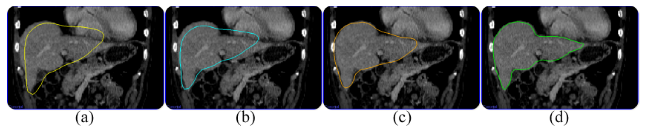
\includegraphics[width=0.7\linewidth]{images/Huang2014_Fig4_v2}
	\caption{The four steps of the liver segmentation framework: (a) liver model location; (b) registration with liver distance map; (c) shape fitting under appearance guidance; (d) free-form deformation. \textbf{©Huang et al. \cite{Huang2014}}}
	\label{Huang2014_Fig1}
\end{figure}


Anter et al. \cite{Anter2014} first detected the liver boundary using fuzzy c-means
clustering based on the gray level local distribution, then refined the
liver segmentation map via connected component analysis. Conze et al. \cite{Conze2017} semi-interactively performed 
the segmentation of the parenchyma, and the separation between 
the active and the necrotic part of the lesions on multiphase CT images.
Images were registered between the different phases using PV phase images as reference, and
supervoxels\footnote{group of voxels sharing the same textural properties}
were computed at different scales using a SLIC (simple linear iterative clustering ) 
algorithm on PV phase images. A random forest was trained 
on a set of retained supervoxels, and used to get a label prediction. 
They proved the value of using dynamic CECT and implementing 
hierarchical multi-scale supervoxels to better segment the liver tissues.\\
It has been proven that methods relying only on intensity are not robust
enough to produce acceptable results especially when dealing with some
primary tumors that present high textural heterogeneity. Prior knowledge
and engineered features were added over time to increase the
performances, but remained sensitive to the size of the dataset used in
the training process, and the amount of interaction to incorporate in
the workflow.
Historically, semi-automatic methods were used for liver tissue
segmentation, while they now tend to be replaced by automatic
techniques, offering reproducibility and fewer interactions with
experts. However, newer methods still suffered when dealing with
pathological livers, often presenting irregular shape or intensity
patterns.
Recently, deep learning has changed the way of comprehending different
computer vision related problems, especially in the medical imaging
field, where state-of-the-art methods rely now on these techniques.

%\emph{Worth also noting that performances were increased for the lesions
%	segmentation, when performed on a restricted liver enveloppe, thus
%	reducing the amount of false positives.}

\section{Deep Learning based semantic segmentation methods}

\subsection{DL applied to the medical imaging}

The main breakthrough brought by DL was its ability to detect
morphological properties in images only by using the pixel intensities
as input, whereas traditional machine learning methods often required
sophisticated hand-crafted features to achieve descent results \cite{Litjens2017, Suzuki2017}. Deep learning networks achieved
state-of-the-art results in many medical-related applications among
which classification, localization, detection, registration and
segmentation \cite{Ker2017}. Even with a small number of
training cases, those performances were realized thanks to architecture
choice, data augmentation or transfer learning \cite{Zheng2018, Hu2018}.
As exposed previously, the automatic segmentation of the tumors brings a
volumetric information, that is more powerful than the diameter only,
and that allows to compute the tumor burden, which has an importance
when estimating the efficiency of a given treatment \cite{Gobbi2004, Bornemann2007, Heussel2007, Kuhnigk2006, Puesken2010, Bauknecht2010}.\\
In this regard, several studies have been conducted to perform automatic
liver and liver lesions segmentation.


\subsection{State-of-the-art DL implementations} \label{subsection:StateOfTheArtDlImplementations}

The different DL studies introduced for the liver tissue semantic
segmentation purpose share some common properties that will be exposed
hereafter. We will fist detail the different types of DL architectures that have been developed to perform this task, before introducing the sequential segmentation concept shared by almost all of the reviewed studies. The details regarding the networks input type, the training strategies, and the inference schemes were then discussed.
Details regarding the reviewed studies can be found in the appendix \ref{detailed-analysis-of-the-dl-semantic-segmentation-reviewed-articles}.

\subsubsection{FCN-based architectures}

The use of fully convolutional networks (FCN) was quickly democratized,
and popular imaging-related architectures such as VGG-16 or AlexNet
were transformed to FCNs by replacing dense layers with convolution
layers \cite{Ben-Cohen, Bellver2017}. An illustration of the resulting architecture is given in the figure \ref{Bellver_FCN}. 

\begin{figure}[th!]
	\centering
	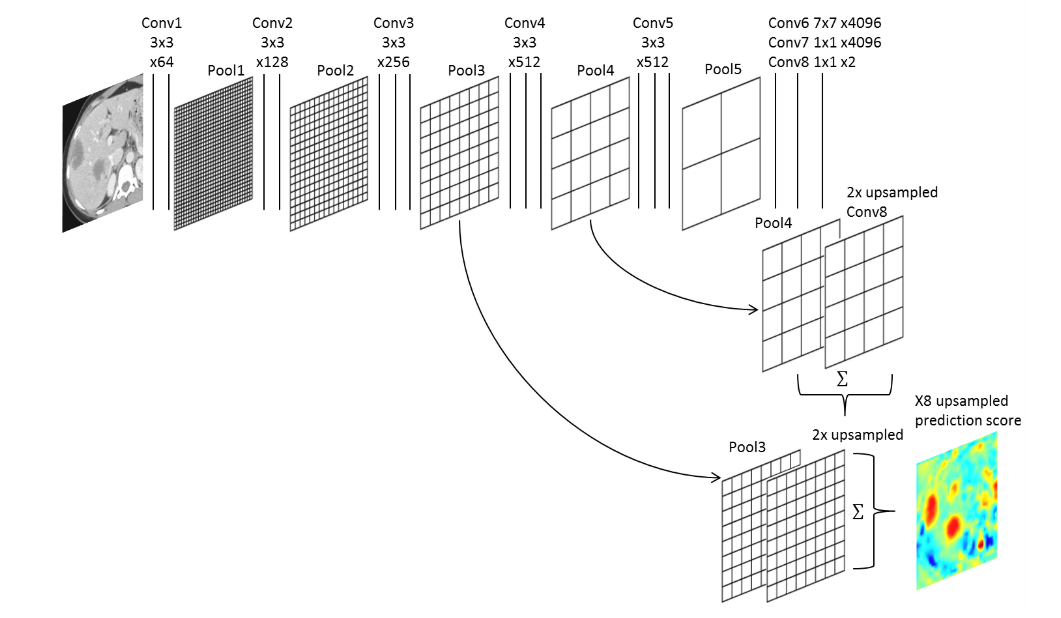
\includegraphics[width=0.7\linewidth]{images/image3}
	\caption{Example of a FCN architecture implemented to perform the liver tumor segmentation task, as described by \textbf{©Bellver et al. \cite{Bellver2017}}}
	\label{Bellver_FCN}
\end{figure}


The FCN allows an architecture to predict as output an object having the
same size as the input. Those architectures were perfectly suitable for
the required segmentation tasks.\\
The most recent studies showed a predominance for U-Net like networks \cite{Vorontsov2018, Yuan2017}. The U-Net was
introduced by Ronneberger et al. \cite{Ronneberger2015} initially for the segmentation of cells
in microscopic images. An overview of its architecture is given in the
figure \ref{U_Net_Figure}. It consists of two parts, the first one where the
information of the image is compressed, going from the extraction of
low-level features, to the extraction of more semantic-related features,
and the second part where the information is resampled back to the
original image resolution. The main advantages of this architecture
reside in the fact that it allows the network having both the input and
the output sharing the same resolution, and also the so-called
\emph{skip-connections} that were introduced to reinject the features
learned from the contraction part, in the decoding part.

\begin{figure}[th!]
	\centering
	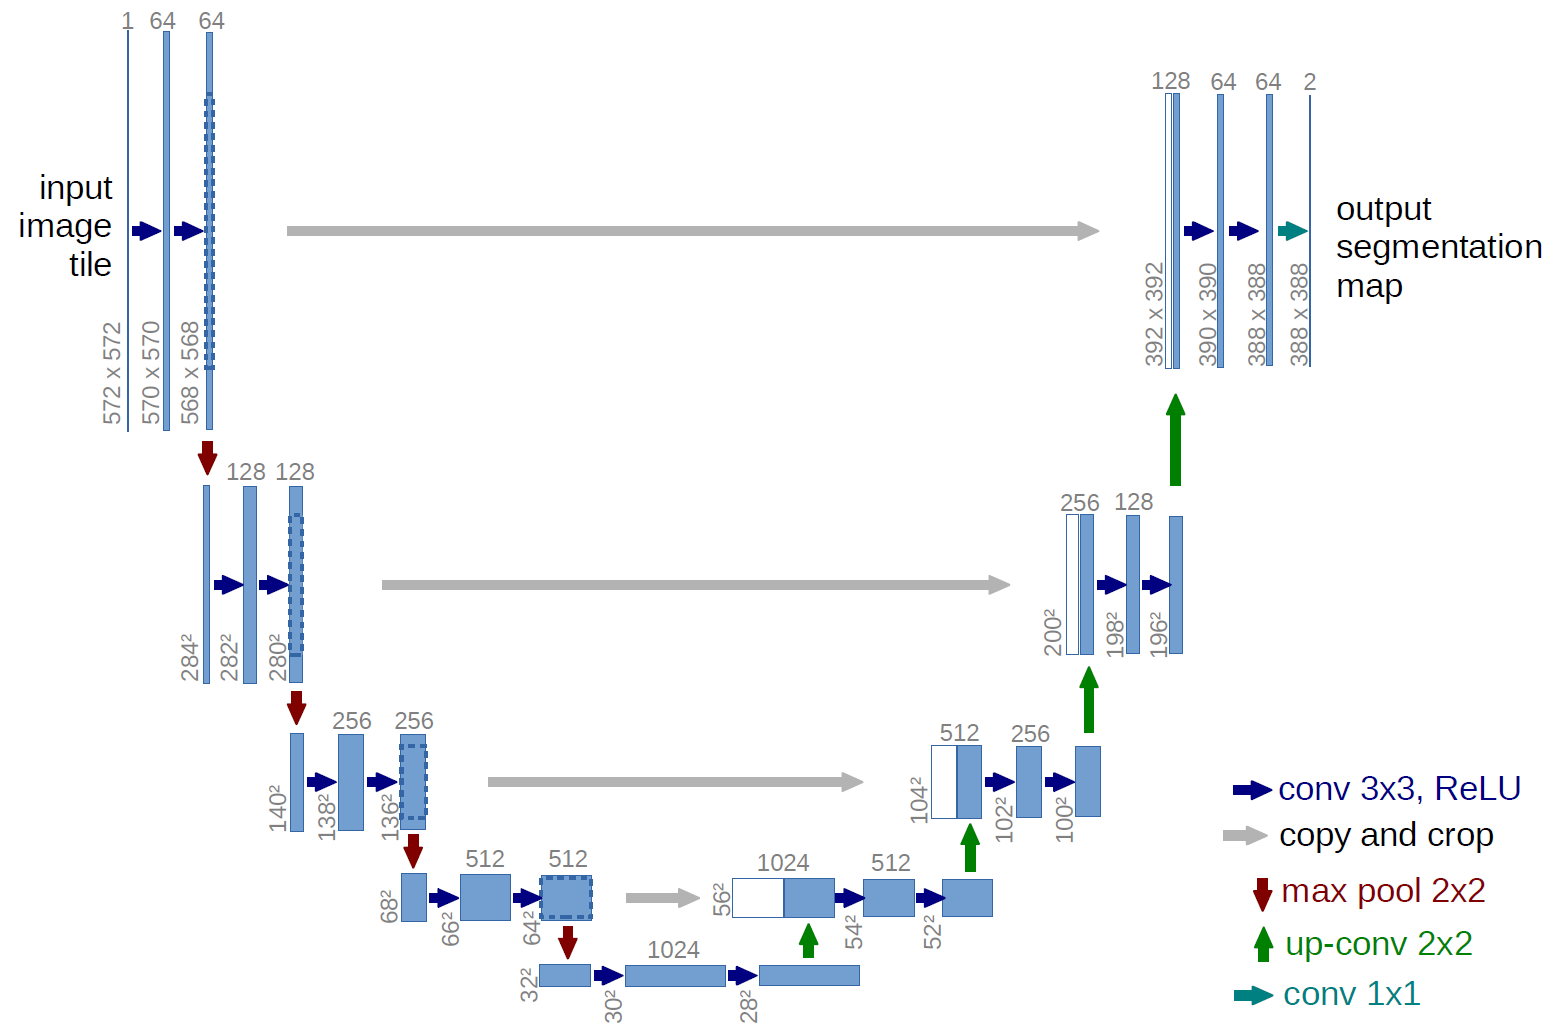
\includegraphics[width=0.7\linewidth]{images/u-net-architecture}
	\caption{U-Net architecture as originally implemented and described by \textbf{©Ronneberger et al.\cite{Ronneberger2015}}}
	\label{U_Net_Figure}
\end{figure}

Two other well-known architectures named ResNet and DenseNet were
implemented in some other studies, either alone or in combination with
the U-Net \cite{Han2017, Chlebus2018, Bi2017, Kaluva2018, Li2018}.\\
The residual network (\emph{ResNet}) developed by He et al. \cite{He2015} in
2015 introduced the concept of residual connections, that help deep
networks overcome the gradient vanishing problem. At each stage of the
network, identity connections, as illustrated in the figure \ref{ResidualConnection_Fig}, allow the
information to be passed from one block to the following, so that early
features are not lost.

\begin{figure}[th!]
	\centering
	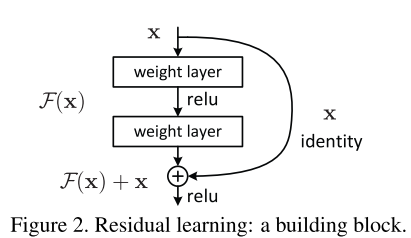
\includegraphics[width=0.4\linewidth]{images/image6}
	\caption{Residual connection as described by \textbf{©He et al. \cite{He2015}}}
	\label{ResidualConnection_Fig}
\end{figure}

Densely connected networks (\emph{DenseNet}) introduced by Huang
et al. \cite{Huang2017} in 2017 share the same motivation of allowing early layers
features being kept all throughout the network. Contrary to the ResNet,
the DenseNet requires less parameters and enables faster computation
since it uses concatenation whereas ResNet added features map that
needed to be kept \cite{Huang2017}. Example of DenseNet
architecture built for a classification task is depicted in the figure \ref{DenseNet_Fig}.
\begin{figure}[th!]
	\centering
	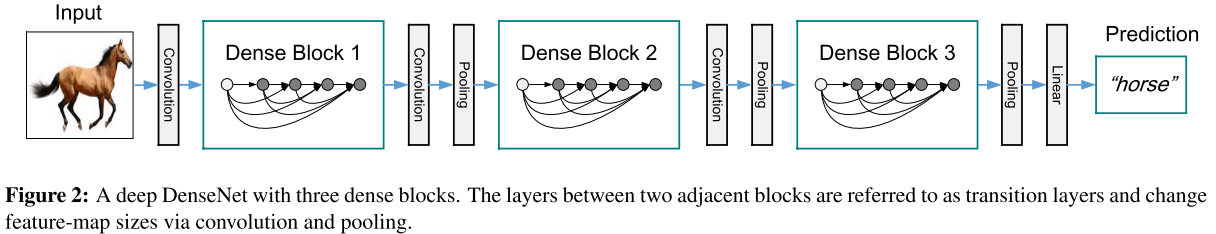
\includegraphics[width=0.9\linewidth]{images/image32}
	\caption{DenseNet architecture as initially described by \textbf{©Huang et al. \cite{Huang2017}}}
	\label{DenseNet_Fig}
\end{figure}


\subsubsection{Cascaded architectures}

To segment the liver and the lesions it might contain, the vast majority
of the studies used a cascaded architecture where a coarse liver
segmentation is performed, before either being refined \cite{Yuan2017} or directly used to segment the lesions \cite{Han2017, Li2018, Kaluva2018, Ben-Cohen, Christ2017}. An example of cascaded architectures is
given in the figure below. 
\begin{figure}[th!]
	\centering
	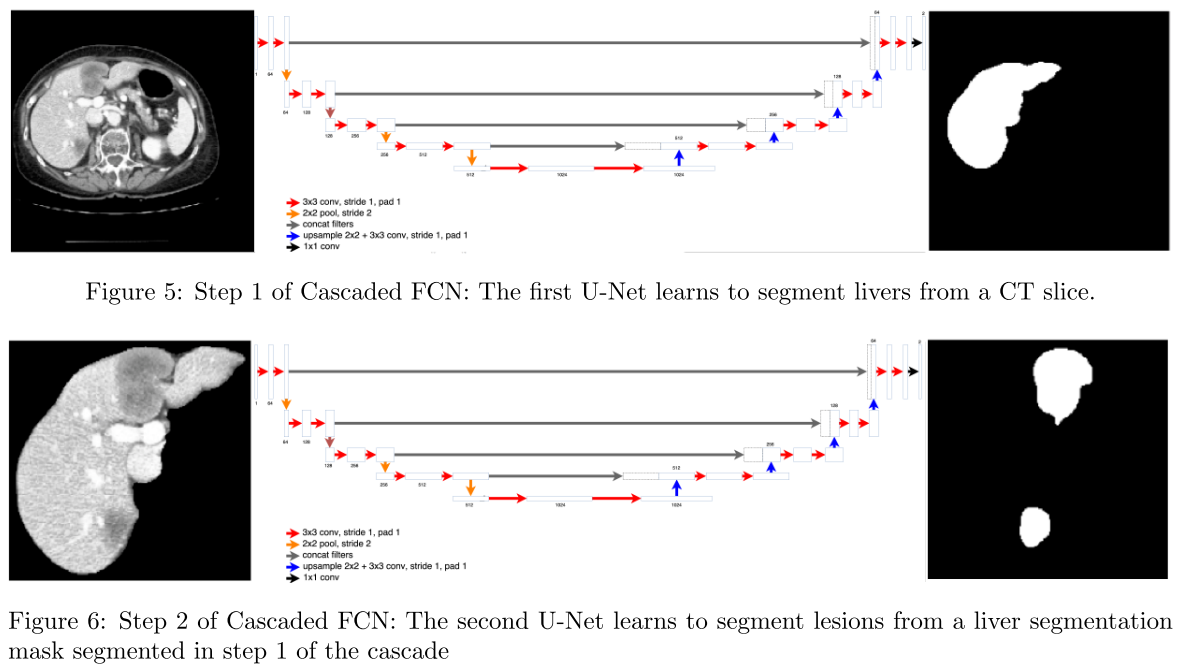
\includegraphics[width=\linewidth]{images/image35}
	\caption{Cascaded liver and lesion segmentation architecture as initially implemented by \textbf{©Christ et al. \cite{Christ2017}}}
	\label{Cascade_Christ}
\end{figure}

Interestingly, some studies decided to extract features before combining
them to get a final segmentation map. For example, Bi et al.
proceed first to an extraction of both liver and lesion features, before
combining them with the original image to perform a pixel-wise
categorical classification, as illustrated in the figure \ref{Bi2017_Fig2} \cite{Bi2017}.

\begin{figure}[th!]
	\centering
	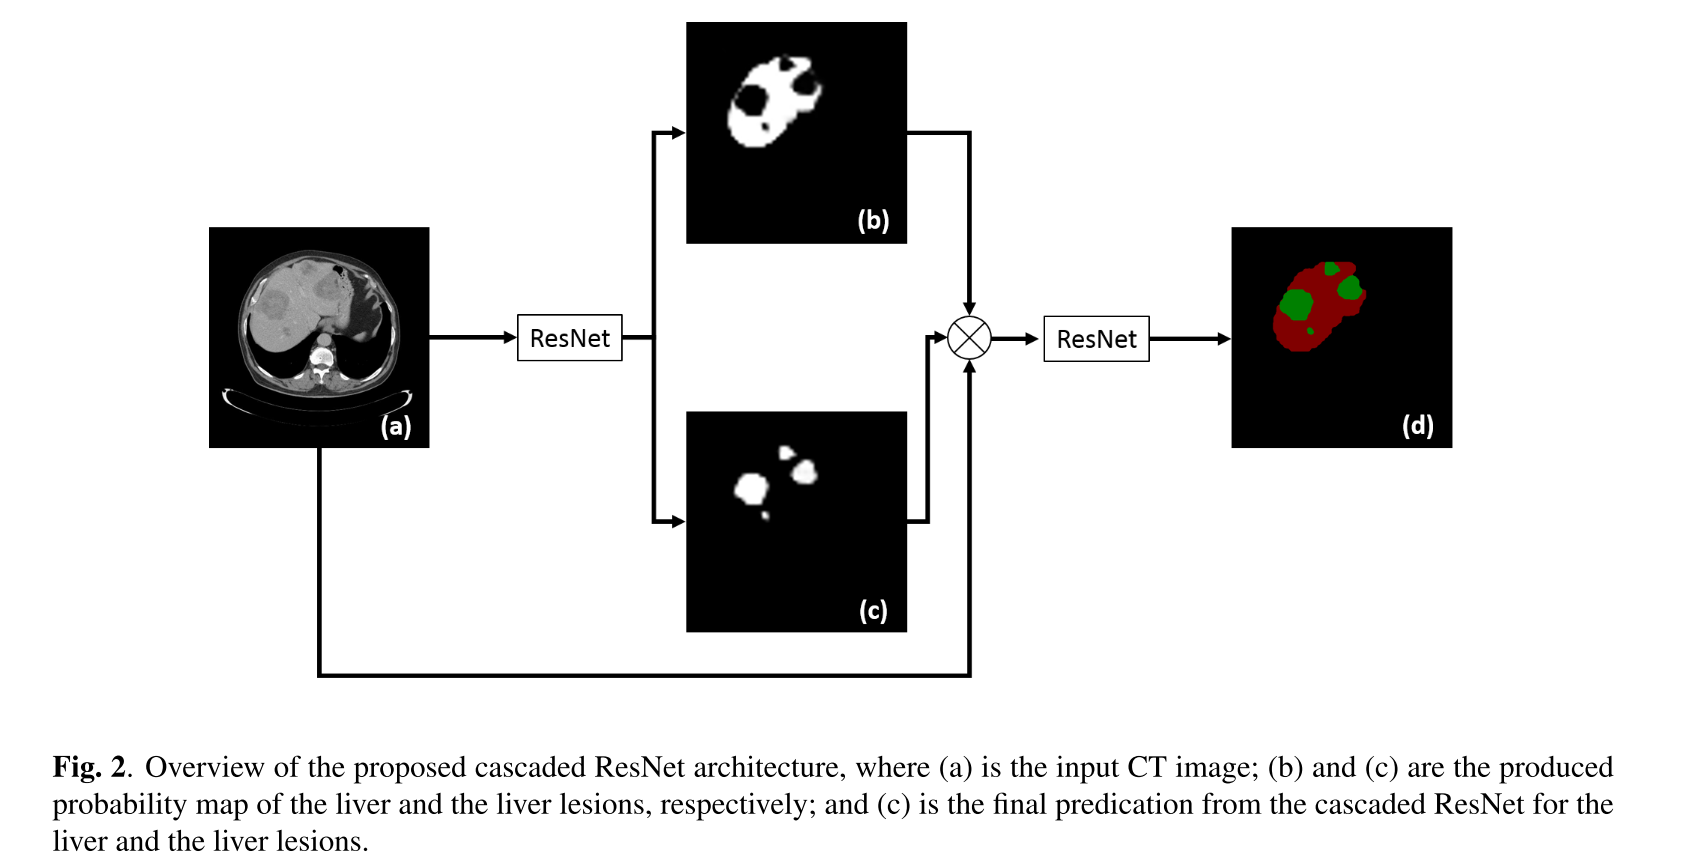
\includegraphics[width=0.7\linewidth]{images/image27}
	\caption{Custom cascaded architecture implemented by \textbf{©Bi et al. \cite{Bi2017}} where the liver and lesions features are first extracted before being combined to produce the final segmentation map }
	\label{Bi2017_Fig2}
\end{figure}


Whereas Vorontsov et al. \cite{Vorontsov2018} separated the extraction of liver
features and lesion features, as detailed in the figure \ref{Vorontsov2018_Fig1}. They
added a classifier at each step which used features concatenated from 3
adjacent slices to get a segmentation of the middle slice.

\begin{figure}[th!]
	\centering
	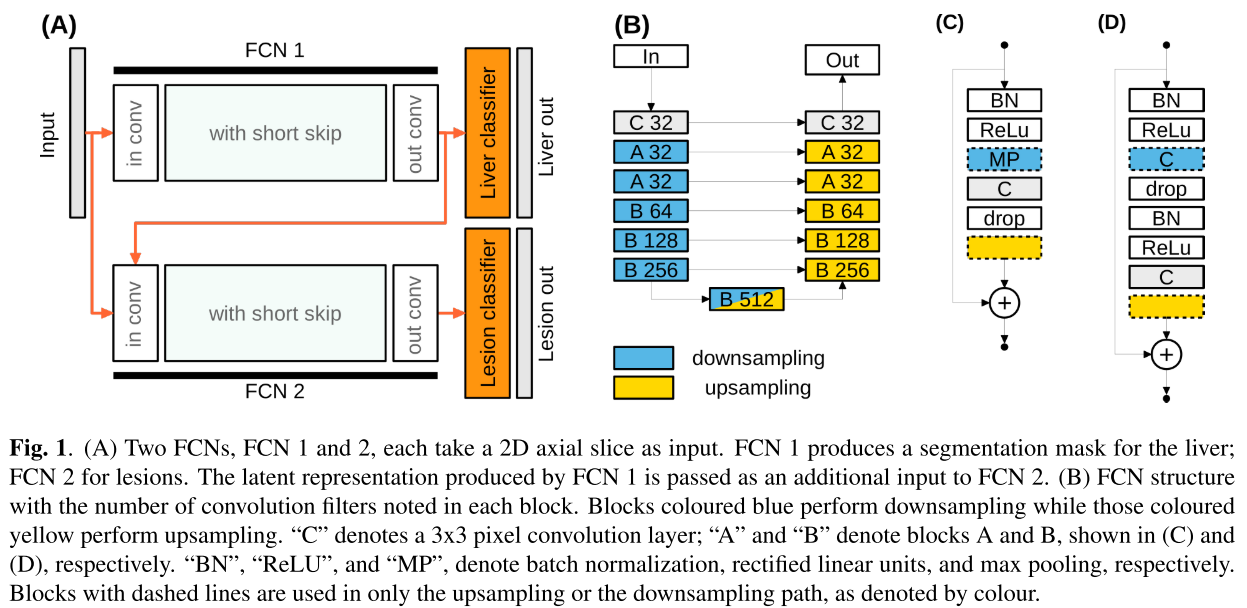
\includegraphics[width=0.7\linewidth]{images/image17}
	\caption{Architecture implemented by \textbf{©Vorontsov et al. \cite{Vorontsov2018}} where the liver and lesions features are computed separately before being combined using a classifier }
	\label{Vorontsov2018_Fig1}
\end{figure}


\subsubsection{Input type (2D, 2.5D, 3D, patches, multiphase)}

The first deep-learning related study that performed the semantic
segmentation of the liver or its lesions, used patches as input.
Li et al. \cite{Li2015} trained a classification model where patches were
considered as positive if at least 50\% of its pixels are tumoral.
Details of their network are given in the figure \ref{Li2015_Patch_fig}.

\begin{figure}[th!]
	\centering
	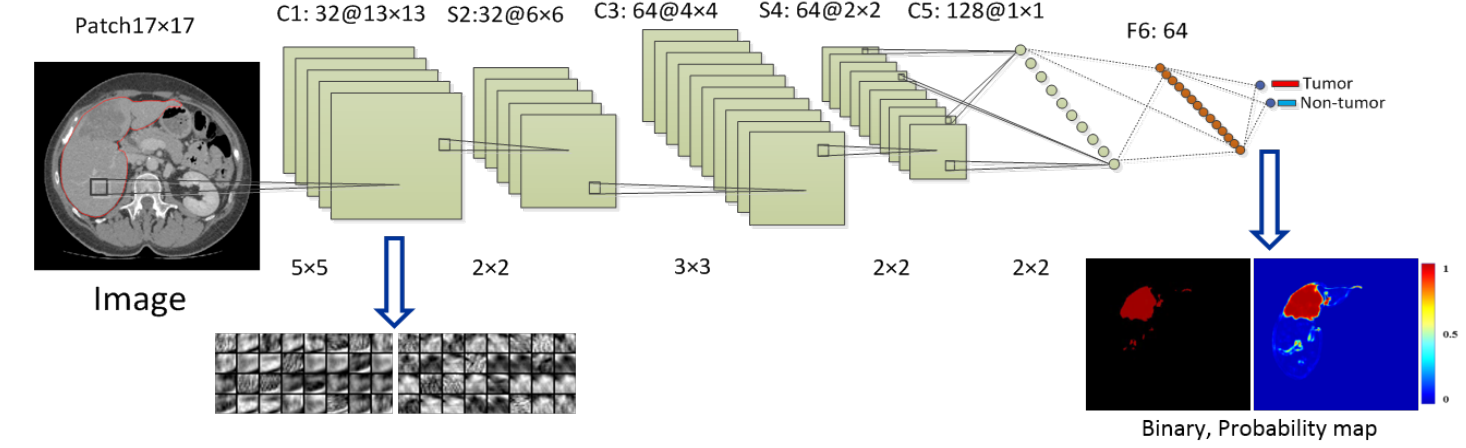
\includegraphics[width=0.7\linewidth]{images/image2}
	\caption{Patch-wise architecture as detailed and described by \textbf{©Li et al. \cite{Li2015}}}
	\label{Li2015_Patch_fig}
\end{figure}


Later, Frid-Adar et al. \cite{Frid-adar2017} also implemented a patch-based
segmentation, but by separating \emph{non-lesion} patches on whether
they are located in the \emph{liver interior} or in the \emph{liver
	boundary}. The classification was performed through a multi-scale
approach, followed by a CNN-based FP reduction step.\\
However, the majority of the studies implemented a slice-by-slice
segmentation \cite{Chlebus2018, Kaluva2018, Bi2017}, whereas some others chose to introduce volumetric
consistency by using 3 or sometimes 5 adjacent slices as input in a
2.5D-manner \cite{Han2017, Yuan2017, Bellver2017}.\\
Worth noting that only a few studies incorporated 3D layers in
their architecture, such as Li et al. who computed 3D
inter-slice features in 12-slices blocks all along the different CT
scans \cite{Li2018}. Rafiei et al. \cite{Rafiei2018} decided to incorporate 3D layers only in
the encoding part of their \emph{3D-2D-FCN} model. The connection
between the encoding part and the decoding part was done by custom
\emph{skip connections} to concatenate the middle slice of the 3D volume
with its corresponding 2D features map in the decoding part. Dou
et al. were the first to build an entire 3D network with large kernels,
and had intermediate supervised layers to combat the gradient vanishing
problem \cite{Dou2016}. Details of their network are given in the figure \ref{Dou2016_3Darchitecture}.

\begin{figure}[th!]
	\centering
	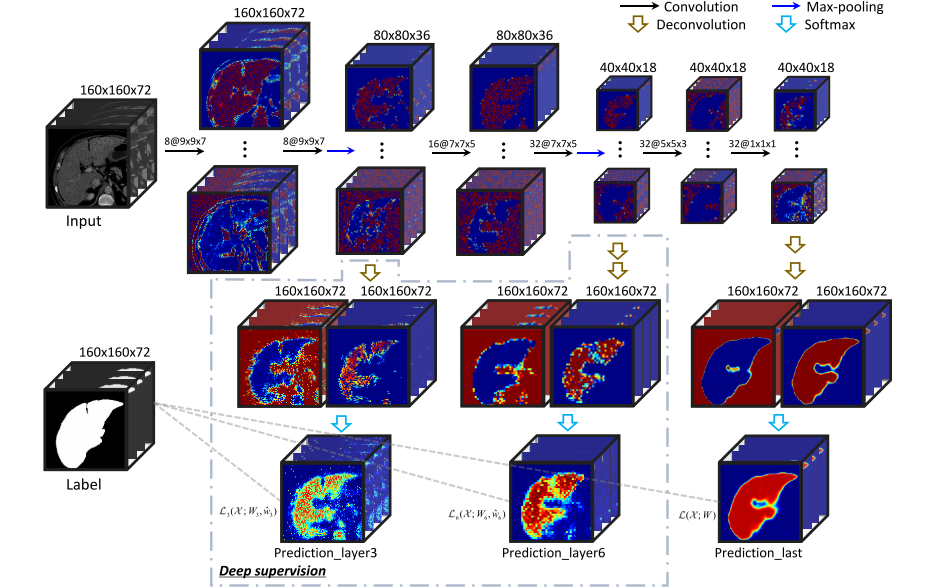
\includegraphics[width=0.7\linewidth]{images/image30}
	\caption{Full 3D architecture as detailed and implemented by \textbf{©Dou et al. \cite{Dou2016}}}
	\label{Dou2016_3Darchitecture}
\end{figure}

Concerning the incorporation of temporal information, Sun et
al. were the first to utilize multiphase information during the
DL-driven automatic segmentation of liver lesions \cite{Sun2017}. One FCN network per
channel was trained to extract features before they were merged through
a features fusion layer.

\subsubsection{Training strategies (pre-processing, pre-trained networks\ldots{})}

Regarding the training strategies, no real consensus can be established.\\
Concerning the pre-processing steps, the majority of the studies decided
to perform the liver coarse segmentation on a down-sampled
representation of the images to limit the computational cost, before
using the original resolution to perform the lesion segmentation in
order to not lose any details \cite{Li2018, Han2017, Yuan2017, Kaluva2018, Vorontsov2018}.\\
Data normalization was also commonly applied after clipping the HU
intensities to a given range, but no consensus can be deduced concerning
the clipping range. Interestingly, Kaluva et al. decided to
apply three different windowing ranges to the original image when carrying
out the lesion segmentation which helped the network to better segment the tumor and its boundary that when only one range was applied.
Almost all the reviewed studies performed data augmentation to
artificially increase the size of the dataset, by most of the time
employing classical geometrical transformations such as rotations,
flips, ships, scalings or elastic deformations \cite{Frid-adar2017, Ben-Cohen, Rafiei2018, Christ2017, Li2018, Han2017, Yuan2017, Bellver2017, Bi2017, Vorontsov2018}.

It is also worth noting that no consensus can also be deduced regarding the
training from scratch or the application of fine-tuning after
pre-training the architecture on another dataset such as ImageNet \cite{Bi2017, Bellver2017, Christ2017} .The same differences are remarkable for the choice of slices to
keep during the training. Yuan et al. and Kaluva et al. decided to keep only liver slices plus a certain margin to train the
liver segmentation network, whereas only slices presenting one or
multiple lesions were used to train the lesion segmentation network \cite{Yuan2017, Kaluva2018}.
Bi et al. selected half of the slices to present both the liver
and the lesions, whereas none of them were present in the other half \cite{Bi2017}.
The type of slices chosen is directly linked to the loss function used
to train the network, where some studies implemented a weighted version
of the cross entropy (categorical or binary) \cite{Han2017, Bellver2017, Ben-Cohen, Christ2017}, and some others decided to directly associate the target metric
with the loss function through the Dice or Jaccard distance \cite{Yuan2017, Chlebus2018, Vorontsov2018}

\subsubsection{Inference schemes (post-processing, ensemble learning)}


Finally, the inference schemes present also some differences among the
different proposed methods. \\
The vast majority of the studies applied a post-processing step to
refine the obtained liver segmentation by extracting the largest
connected component \cite{Li2018, Han2017, Yuan2017, Bellver2017, Kaluva2018}. They
also often took advantage of the cascade paradigm where lesions
activations outside of the predicted liver can be removed \cite{Li2018, Yuan2017, Vorontsov2018}. In other studies, the reduction of the FP
(\emph{False Positives}) was done through an additional classifier
filtering the different lesions candidates. Chelbus et al. \cite{Chlebus2018} for
example implemented an object based random forest classifier,
Bellver et al. proposed a patch-based lesion detector as
depicted in the figure \ref{Bellver_predResults} \cite{Bellver2017}, whereas Frid-Adar et al. integrated an
additional CNN designed to detect FP \cite{Frid-adar2017}.

\begin{figure}[th!]
	\centering
	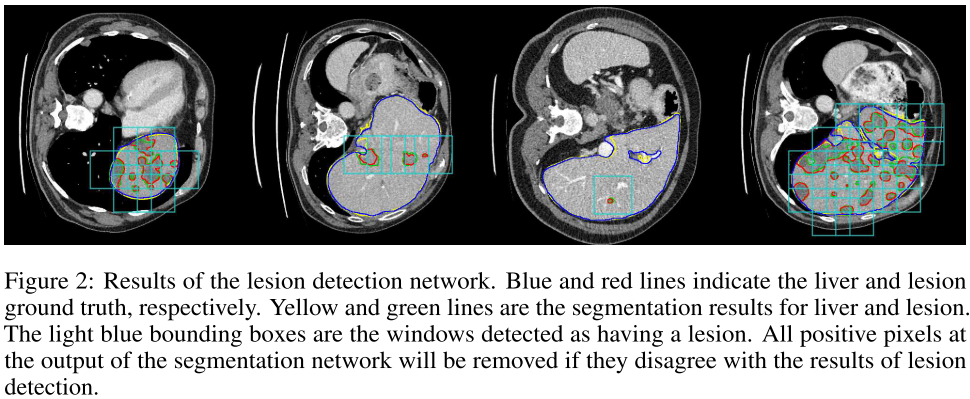
\includegraphics[width=0.7\linewidth]{images/image25}
	\caption{Example of lesion segmentation results, as reported by \textbf{©Bellver et al. \cite{Bellver2017}}}
	\label{Bellver_predResults}
\end{figure}


Some other studies decided to add a more sophisticated step by
implementing Conditional Random Fields (CRF) \cite{Christ2017, Rafiei2018, Dou2016}, however, these models
tend to be difficult to train, and may also
increase the inference time.

The combination of different networks in a so-called
\emph{ensemble-learning} way was also commonly realized by the different
studies. Yuan et al. combined the different networks obtained
through a cross-validation process to give the final segmentation \cite{Yuan2017}.
Whereas Chlebus et al. trained one network per axis \cite{Chlebus2018}. Bi et al. decided to train different networks following a
multiscale-strategy \cite{Bi2017}, and Vorontsov et al. trained networks on
differently oriented images \cite{Vorontsov2018}.

\subsubsection{Conclusion}

As exposed previously, no real consensus can be found to design a
generic DL-related liver tissue semantic segmentation method. However,
the state-of-the-art studies share some common properties such as their
cascaded architecture, the use of both pre- and post-processing or the
use of FCN-based networks as basis.
The different teams that participated in either the MICCAI17 or ISBI17
LITS challenge were reviewed by the organizers, who came to the same
conclusions \cite{Bilic2019}.
They also realized that the best tumor-segmentation results were
obtained for large lesions, and within a specific lesion-liver HU
difference interval (a difference between -10 and -60).
They also noticed that top-ranked methods used some 3D approaches in
their architecture\textbf{,} showing perspectives to capture the whole
volume context in the future. They are planning to organize again the same
type of competition in the future, by particularly providing multiple
ground truths and potentially splitting the lesion segmentation task
into large and small lesions, since current methods still struggle in
segmenting the small lesions.

More recent DL-related studies have been using publicly available
databases such as LITS as a way to compare themselves to
state-of-the-art methods. As a matter of facts, the key common elements
that have been proposed previously served as a basis for new studies.

In the following section, we will present our experiments that were conducted to automatically perform the semantic segmentation of the liver and its potential tumors. Inspired by the above mentioned work, a sequential architecture consisting of several specialized networks was trained by considering the dynamic of the liver thanks to contrast-enhanced CT images. 
% Copy in Perspectives


%Jin et al. for example proposed a network that
%integrated both U-Net and attention residual mechanism to proceed the
%segmentation of both the liver and the lesions \cite{Jin2018}.
%The residual attention mechanism has been introduced in 2017 by Wang et al. to perform image classification, with the idea that attention mechanism
%can help the network focusing on specific parts of the image \cite{Wang2017}.
%The study from Jin et al. was the first to use the attention mechanism
%for semantic segmentation purpose. On the hidden test set of LITS, they
%outperformed a lot of 2D-based methods, but were still far from the
%top-ranked teams \cite{Jin2018}.
%
%However, new paradigms such as the self-attention mechanism, in
%combination with state-of-the-art 2D and 3D architectures are certainly
%an avenue for the improvement of the automatic liver and tumors
%segmentation tasks \cite{Chen2019}.


\section{Semantic segmentation applied to the study of HCC}

As explained previously, state-of-the-art deep learning techniques allow
modern hardware to perform automatic segmentation of both the liver and
its structures with a precision close to the one obtained by the experts
themselves.
In this section, we will first describe the implemented
networks and the different used datasets, before presenting the experiments.
As described previously, no real consensus was made regarding the
design of the DL-related semantic segmentation studies, so we decided to
launch several experiments on selected datasets to determine the impact
of the training strategies on the performances of the networks.
After selecting an optimal set of hyperparameters, we evaluated the
advantages brought by a cascaded architecture, and the way to implement
it, before describing the way to incorporate the multiphase information
in our architecture.
The results and the conclusions of this work were presented in the
literature \cite{Ouhmich2019}.


\subsection{Motivations}

We implemented different architectures to validate the hypothesis that
current deep networks can perform automatic delineation of both the
liver and its tumors. We also proved that incorporating the dynamic information through the use of contrast-enhanced images can improve the performances of the network thanks the specific wash-in wash-out mechanism. 
The features computed by the deep networks will further be used in a
radiomics purpose.
It it worth noting that we are the first to automatically delineate HCC on multiphase CT images using a DL architecture.



\subsection{Cascaded architecture}

Even though no consensus was made regarding existing methods, we noticed that
several studies implemented a sequential pipeline that can be modeled as
cascaded architecture. The cascade consists in several networks trained
to perform a specific simpler task, and that are sequentially connected, to
provide a final annotation map. In our case, the goal is the
segmentation of the liver and its internal structures with the
differentiation between parenchyma, and both the active and the necrotic
parts of the hepatic tumor.
Our cascade will consequently be composed of 3 networks, as depicted
in the figure \ref{CARS_Cascade}. The first one will be specialized to segment the liver in
abdominal axial slices, the second will delineate the contours of the
tumor in the predicted liver ROI, whereas the final one will
differentiate between active and necrotic parts within the obtained
tumor ROI \cite{Ouhmich2019}.
Each one of the given networks will share the same \emph{U-Net}
architecture.

\begin{figure}[th!]
	\centering
	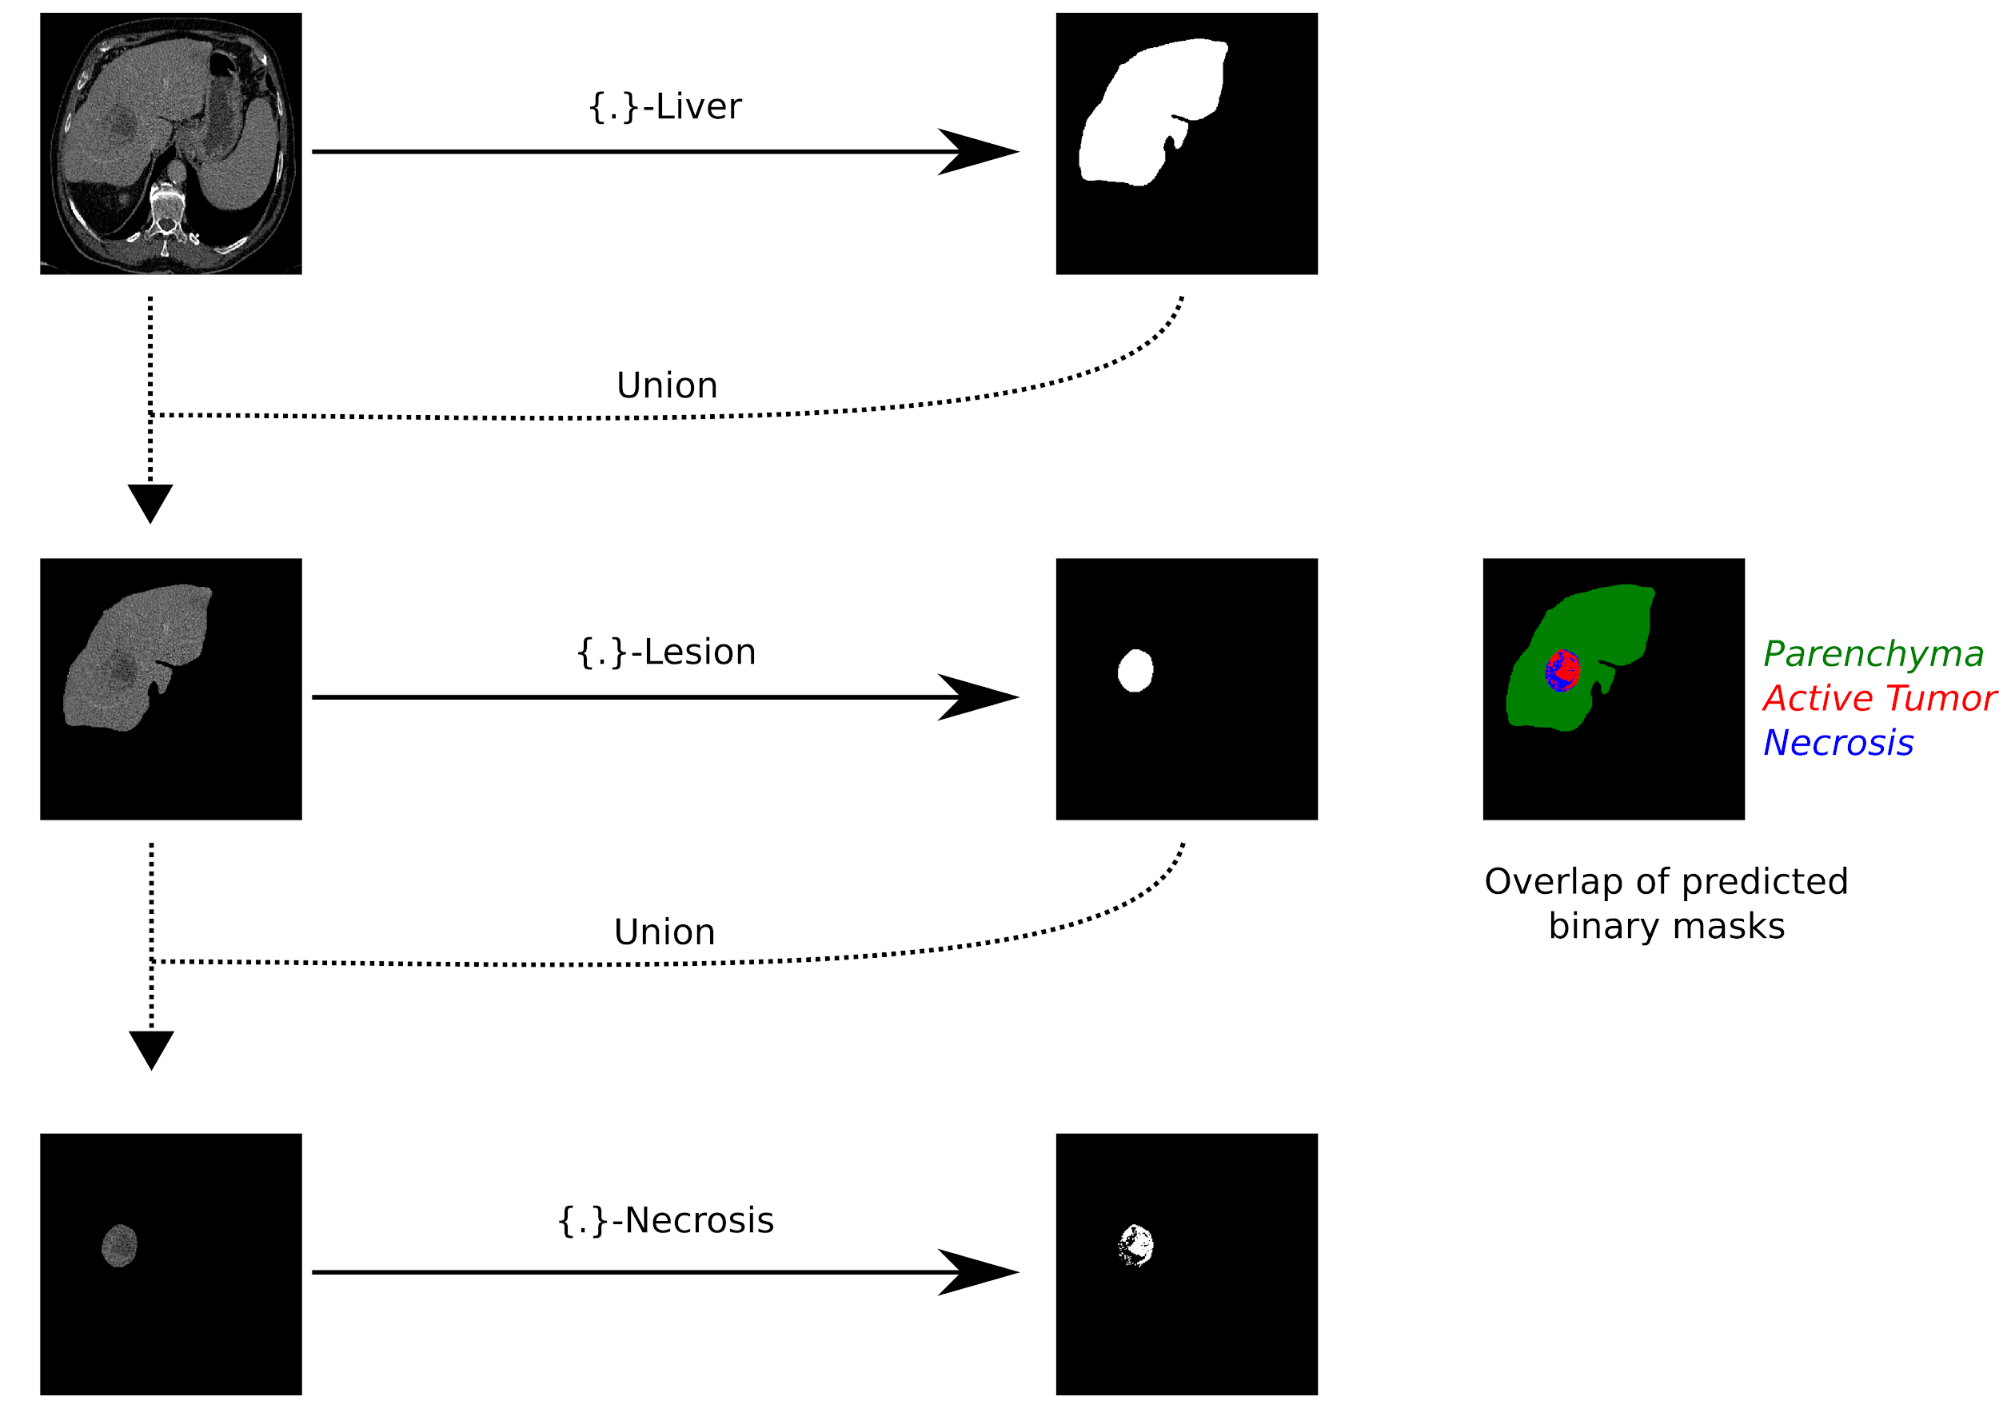
\includegraphics[width=0.7\linewidth]{images/image26}
	\caption{Cascaded network: The first network takes as input a CT image and segments the liver. The resulting segmentation map is used to remove non-liver pixels in the input data of the second network which performs the segmentation of lesions. The last network segments the necrosis within the lesions. The three binary masks are combined in the final segmentation map.}
	\label{CARS_Cascade}
\end{figure}


\subsection{U-Net network}

As a basis architecture, we have decided to implement \emph{U-Net} like
networks because it has been previously used for the semantic
segmentation task, and has proven to give good results even with a
small number of training samples. \\
The original \emph{U-Net} architecture was developed by Ronneberger et
al. \cite{Ronneberger2015} and initially designed for the
delineation of cells in microscopic images. As detailed previously, the
network can be divided into two subparts, a contraction one where the
information contained within the images is compressed, through the
extraction of high to low level features, and a decoding part where the
compressed information is used to reconstruct a high resolution
segmentation. The architecture was initially composed of 19
convolutional layers, with a rectified linear unit function as
activation. The input image had an initial size of $ 512\times512 $ pixels, and
at each stage of the encoding part, 2 convolutional layers are stacked
with an increased number of filters. The initial pair of convolution
layers used 64 filters each, whereas the final stage of the encoding
stage used 1024 filters. After each pair of convolutional layers, a max
pooling layer is applied to halve the spatial dimension of the features
maps. As a result, a $ 30\times30\times1024 $ features map is produced at the
bottleneck of the network. This representation is then reformatted in
the decoding part to obtain a segmentation map with a size equivalent to
the one of the input image. In order to increase the spatial dimension
of the features maps, Up-Convolutional layers are implemented. It is worth
noting that the number of filters used in each of the pair of
convolutional layers is decreased from the bottleneck to the final layer
of the network. The last convolutional layers will map the obtained
features to the final number of dimensions of the segmentation maps,
which will correspond to the number of classes to predict. The final
layer implements a softmax function, to simulate a prediction of
appartenance to each one of the output class.

In comparison to the original architecture, we have implemented
zero-padding convolutions to preserve the image size and obtain a
segmentation map with the same spatial dimension as the input image. We
conserved the same settings as in the original architecture concerning
the number of filters to use at each stage, starting with a pair of
convolutions of 64 filters each, and reaching a $ 32\times32\times1024 $ features map
in the bottleneck part of the network. \\
The same naming-system as in our study will be used
here \cite{Ouhmich2019}. Single-phase elementary networks will be referred to by both the
input phase and the segmentation target, as an example, \pplfont{PV-Lesion} will
refer to the network responsible for the segmentation of the lesion,
with PV phase images as input. The complete \emph{U-Net}
architecture for this specific elementary network is depicted in the figure \ref{CARS_PV_lesion_Fig}.

\begin{figure}[th!]
	\centering
	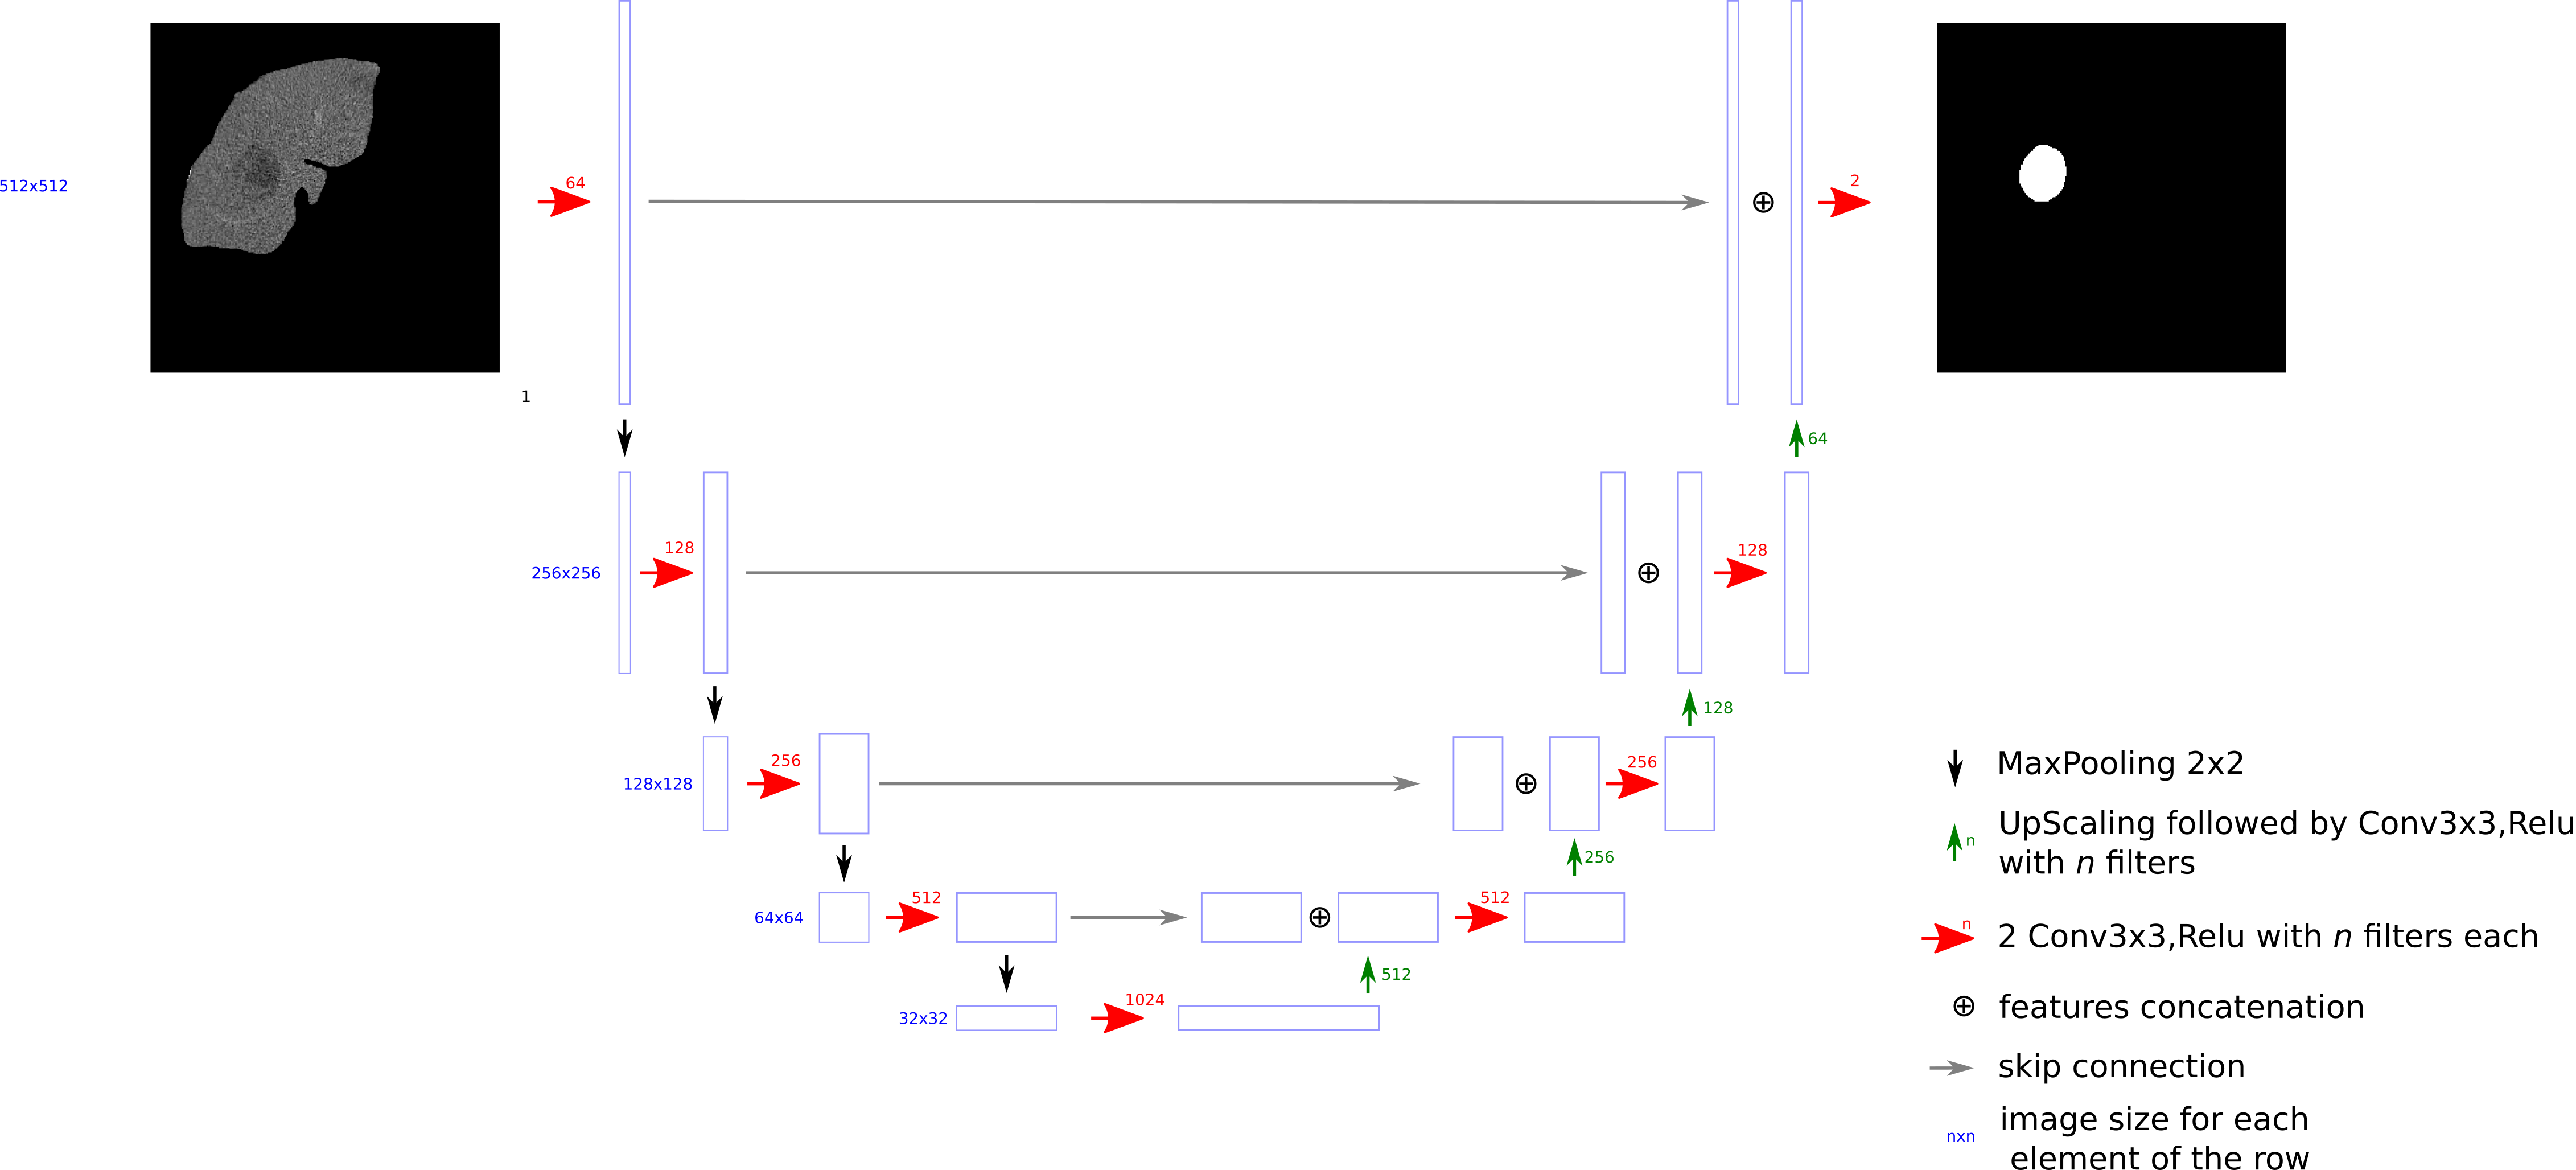
\includegraphics[width=0.9\linewidth]{images/PV_Lesion}
	\caption{\pplfont{PV-Lesion} network used to segment lesions within the liver with a PV image as input}
	\label{CARS_PV_lesion_Fig}
\end{figure}


In order to evaluate the improvements brought by the cascaded
architecture, we also trained the original \emph{U-Net} architecture to
perform simultaneously the whole internal tissues segmentation task. The
same naming system as previously will be used where ``Full'' corresponds
to the simultaneous segmentation task, thus, \pplfont{AR-Full} will refer to the
network dedicated to the segmentation of both the parenchyma, the active
and the necrotic part of the lesions simultaneously, with AR
images as input. An illustration of the network is given in the figure
\ref{CARS_ArFull_Fig}.

\begin{figure}[th!]
	\centering
	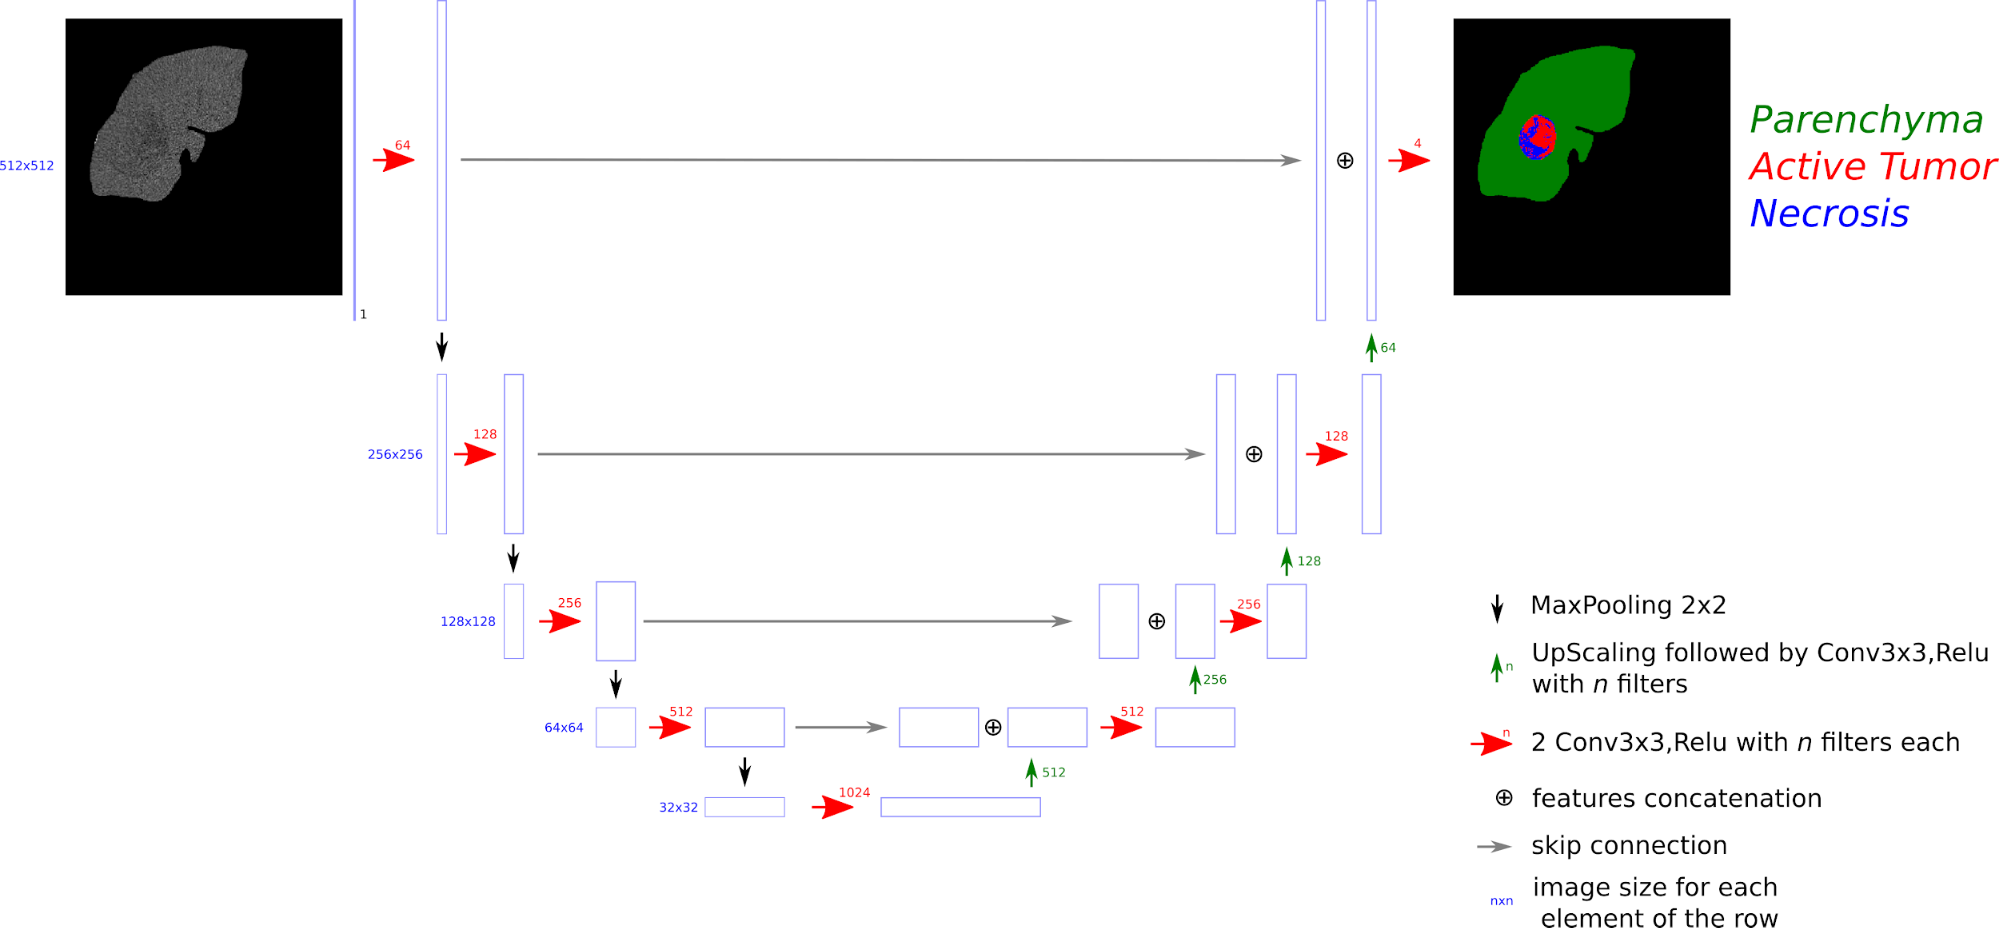
\includegraphics[width=0.9\linewidth]{images/image23}
	\caption{\pplfont{AR-Full} refers to the network trained with AR images as input (values outside the liver are masked), and that outputs a label map, with parenchyma, active and necrotic parts annotated}
	\label{CARS_ArFull_Fig}
\end{figure}


\subsection{Multiphase information}

Only the AR and PV phases were considered in the
multiphase networks because NECT phase images do not provide enough
inter-tissue contrast. \\
In order to incorporate the multiphase information in our pipeline, we
investigated 2 different strategies. The first one, referred to as DMP (Dimensional MultiPhase), consists in concatenating both the
AR and PV images as input to the network (see figure \ref{CARS_DMP_Full_Fig}).
The second one referred to as MPF (MultiPhase Fusion), consists
in performing both the encoding and the decoding separately for each
phase, before merging the output maps (simple addition on the obtained
features maps), as depicted in the figure \ref{CARS_MPF_Full_Fig}.

\begin{figure}[th!]
	\centering
	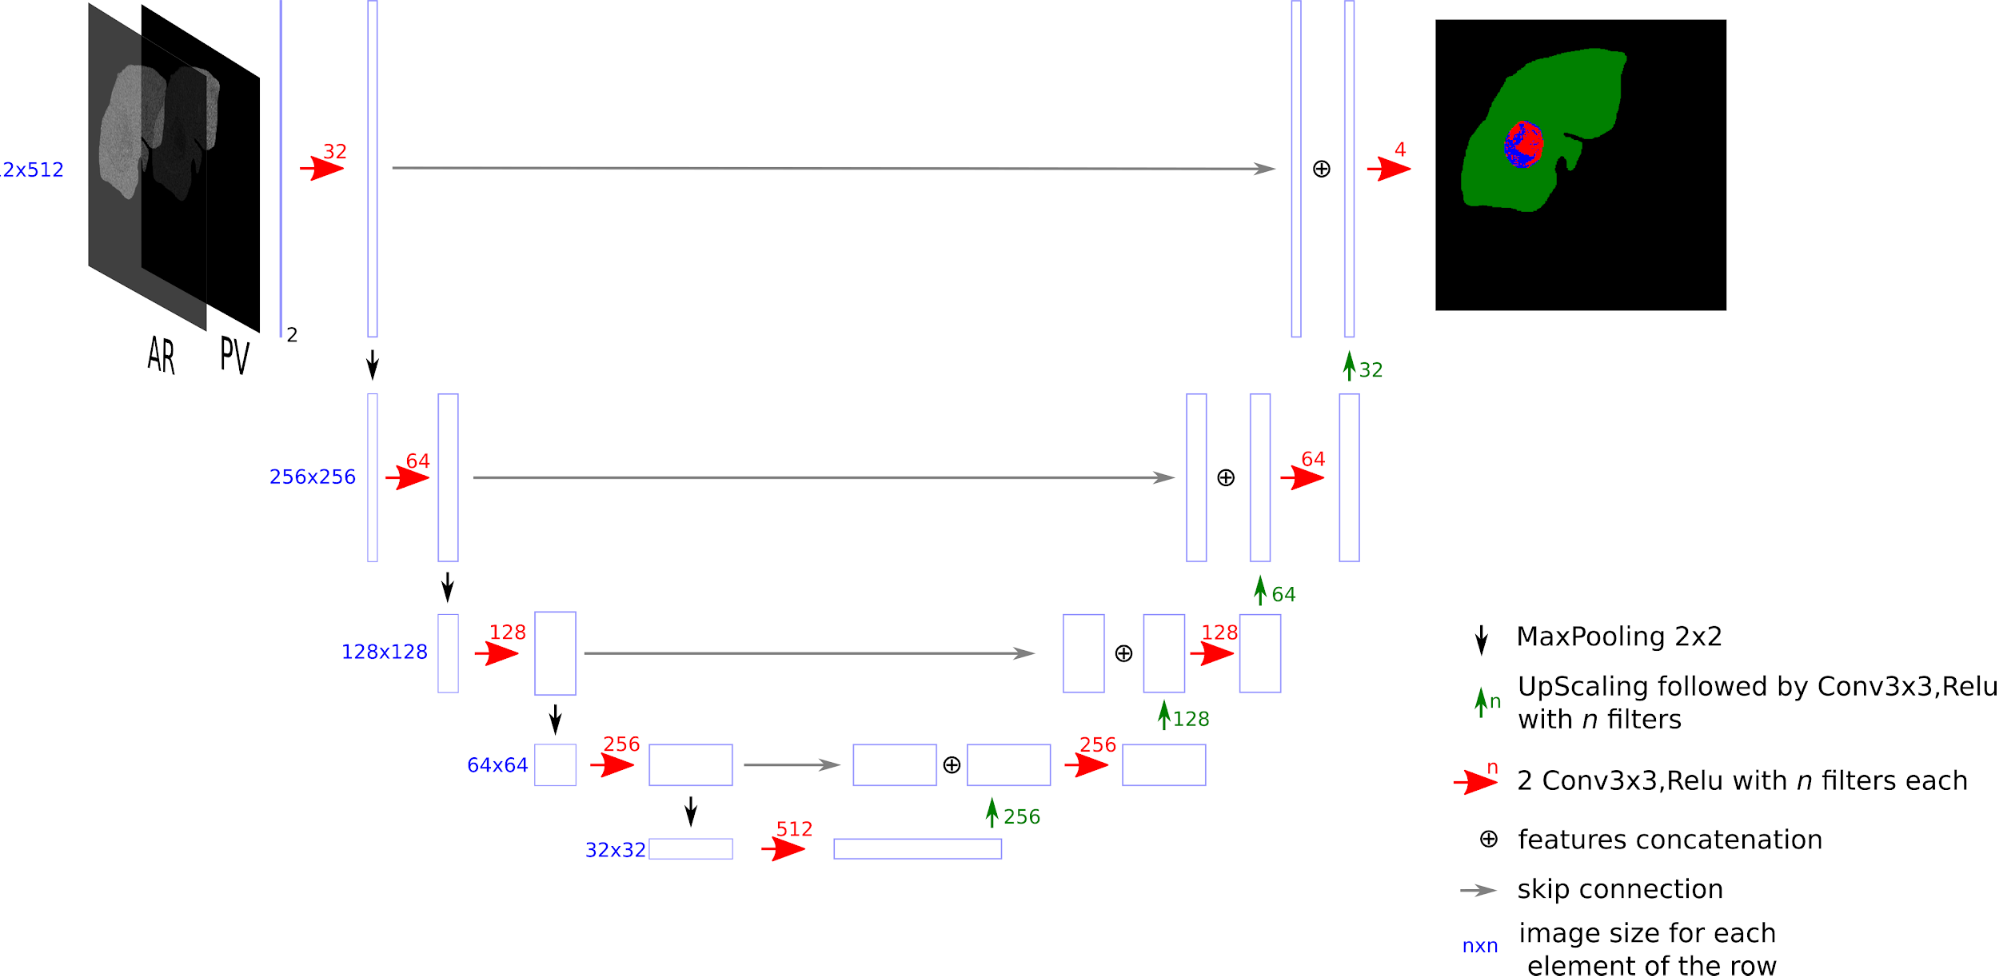
\includegraphics[width=0.9\linewidth]{images/image28}
	\caption{\pplfont{DMP-Full} network that combines the AR and the PV images as an input to segment the parenchyma and both the active and the necrotic parts of the lesions. Here, the two channels are considered as features for the first layer}
	\label{CARS_DMP_Full_Fig}
\end{figure}


\begin{figure}[th!]
	\centering
	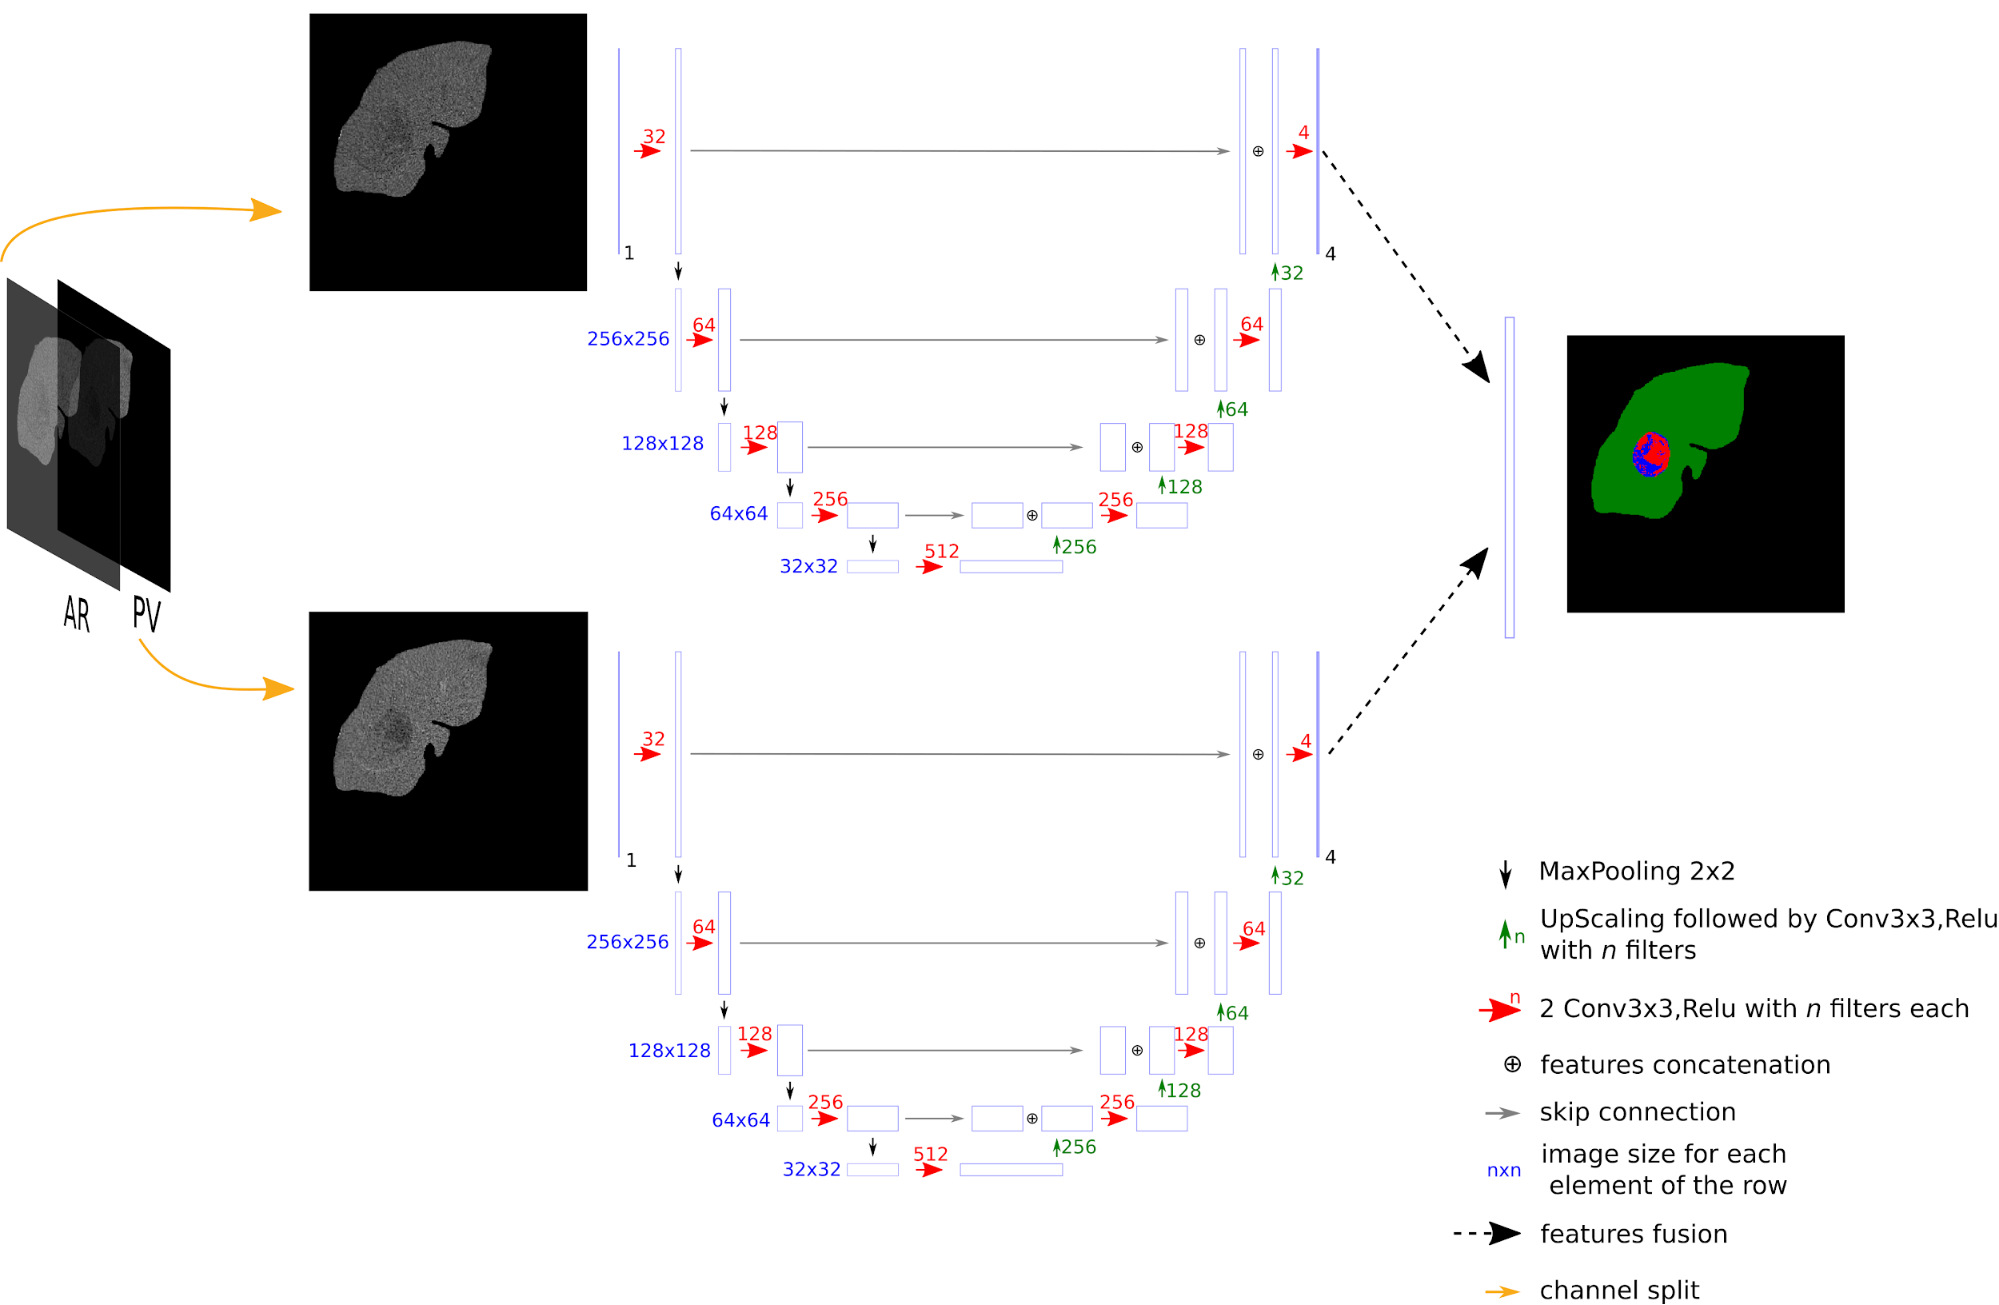
\includegraphics[width=0.9\linewidth]{images/image36}
	\caption{\pplfont{MPF-Full} network: initially, AR and PV images are processed separately. The resulting maps are merged (by simple addition) at the end}
	\label{CARS_MPF_Full_Fig}
\end{figure}





\subsection{Datasets}

The different datasets used in our research work are detailed in the
table \ref{xp_datasets}.

\renewcommand{\arraystretch}{2}
\setlength{\tabcolsep}{7pt}
\newgeometry{top=5mm, left=5mm, right=5mm, bottom=10mm, footskip=5mm, headsep=10mm}

\begin{landscape}
\scriptsize
	\begin{longtable}{l|p{2cm}p{1.5cm}p{1.6cm}p{3cm}p{1.5cm}p{1cm}p{1cm}p{1cm}p{1cm}p{1cm}p{1cm}}\toprule
		\textbf{Db Name} & \textbf{Db retained number of cases} & \textbf{Axial voxel size (mm)} & \textbf{Slice Thickness (mm)} & \textbf{Available contrast-enhanced phases} & \textbf{Contains Tumor} & \textbf{Tumor type} & \textbf{Liver  Ground truth} & \textbf{Tumor Ground truth} & \textbf{Necrosis Ground truth}& \textbf{\#Experts} \\
		\midrule
		\textbf{\lmttfont{TheraHCC-dB}} &104 2D slices &0.66-0.97 &0.7-1.25 &NECT, AR \& PV&Yes &HCC & true & true & true &4 \\
		\textbf{\lmttfont{LITS-dB}}& 131  3D vol. & 0.55-1 &0.45-6 &Single phase images but mixed (AR \& PV)&Yes &Mixed & true & true & false &3 \\
		\textbf{\lmttfont{3DIrcad-dB}}\footnote{Subset of the 3DIrcad-01 presented in the table \ref{publicly_available_datasets} where only the 15 volumes with liver tumors were retained} & 15 3D vol. &0.57-0.87 &1.25-4 &Single phase images but mixed (AR \& PV) &Yes &Mixed & true & true & false &- \\
		\textbf{\lmttfont{TCIA-dB}} \footnote{Subset of the one presented in the table \ref{publicly_available_datasets} where only the 18 exploitable volumes with both AR and PV phases were retained} & 18 3D vol. &0.62-0.90 &2.5-7 &AR\&PV&Yes&HCC & false & true & true &1 \\
		\textbf{\lmttfont{G-dB}} & 79  3D vol. &0.58-0.98 &0.8-5 &AR\&PV&Yes &HCC & false & true & false &1 \\
		\bottomrule
		\caption{Datasets used in our experiments (NECT: Non-Enhanced Contrast CT, AR: Arterial, PV: Portal Venous)}\label{xp_datasets}
	\end{longtable}
\end{landscape}

\renewcommand{\arraystretch}{5}
\newgeometry{vmargin={15mm}, hmargin={30mm,30mm}}   % set the margins 

As we can see in the table, and except for \textbf{\lmttfont{LITS-dB}} and \textbf{\lmttfont{3DIrcad-dB}}
(\textbf{\lmttfont{3DIrcad-dB}} being a subset of the \textbf{\lmttfont{LITS-dB}} \cite{Bilic2019}), they are all different in their construction. Differences can
be found on the annotated areas (chosen sparse slices or entire 3D
volumes) and on the annotated tissues that can be found in the dataset
(some of them only contain ground truth annotations for the liver and
the tumors it might contain such as \textbf{\lmttfont{LITS-dB}}, whereas some others contain
only ground truth annotation for the tumor such as \textbf{\lmttfont{TCIA-dB}}). Another
crucial difference concerns the contrast enhanced phases available in
each dataset (\textbf{\lmttfont{LITS-dB}} contains only single phase images whereas \textbf{\lmttfont{TCIA-dB}},
\textbf{\lmttfont{TheraHCC-dB}} and \textbf{\lmttfont{G-dB}} present multiphasic images). \\
To prove the ability of the deep learning to perform the automatic
segmentation of both the liver and its internal tissues, such as the
parenchyma and both the active and the necrotic part of the tumor, we
first performed our experiments on \textbf{\lmttfont{TheraHCC-dB}} since this database was
previously used for the same task \cite{Conze2017}, because it
presents multiphase images and finally because this is the only
available dataset with complete ground truth for both liver parenchyma,
active and necrotic part of the tumors. \\
\textbf{\lmttfont{TheraHCC-dB}} is composed of images from seven patients, all suffering
from \emph{HCC} and who underwent CECT (Contrast-Enhanced
Computed Tomography) examinations, resulting in a total of 13 CT
sequences. \\
More details about the standard CECT examination protocol can be
found in the chapter \ref{ct-and-mr-imaging}. In our case, images were acquired at 4 different
moments: one before the injection of the contrast medium (NECT:
Non Enhanced CT) , and the 2 others after the injection to reflect both
the arterial (AR) (\textasciitilde{}20-25s after injection) and
the portal venous (PV) phases (\textasciitilde{}60-70s after
injection).\\
Eight regularly sampled slices across each one the 13 sequences were
segmented by 4 experts, resulting in 104 labeled slices. \\
The segmentation maps obtained from each one the 4 experts were fused
using the STAPLE algorithm to reach a consensus map \cite{Warfield2004}.


\subsection{Experiments}

\subsubsection{Data pre-processing}

The first task to implement in this study was the inter-phase
registration so that environmental effects, such as respiratory motions,
will not affect the performances of the networks, and to ensure that a
given voxel is at the exact same position for the different CECT
volumes of a patient. The registration was performed using a
diffeomorphic deformable registration algorithm, where the PV
images were used as reference, since they contained the original expert
annotations \cite{Avants2008, Conze2017, Ben-Cohen, Christ2017}. \\
Another bias that can affect the deep semantic segmentation networks
training is the heterogeneous image sizes and voxel resolutions present
within the training images.
To avoid this bias, it has been decided to scale them so that they all
have a $ 512\times512 $ axial size \footnote{Either cropping or padding was performed so that the images have the same size} and an isotropic voxel resolution of $ 0.97 \text{mm}^2 $. \\
The data normalization is another aspect that needs to be considered
before feeding the images in the deep network. In order to reduce the
effect of extreme values from regions present in the tomographic images
(such as the bones or the air), and to enhance the intensity of the
liver voxels, we first clipped the \emph{HU} values to be in the range
$ \left[-100, 400\right] $ , corresponding to the most commonly 
observed liver intensities range. The retained intensities were finally mapped to
the interval $ \left[0, 1\right]$ \footnote{DL studies usually tend to perform 
data standardization but here HU values are already normalized. 
The used range helps us to avoid potential bias caused by images acquired at a delayed phase with a different contrast}.

\subsubsection{Training}

In order to validate our hypotheses, we have decided to first run
experiments on the \lmttfont{3DIrcad-dB} to set the most crucial hyperparameters
such as the learning rate, the decay, the depth of the network or the
type and the amount of data augmentation.
The selection process is detailed in the \textbf{Appendix}, and here is the list of the chosen hyperparameters:

\begin{itemize}
	\item Lr: 1e-4
	\item Decay: 1e-4
	\item Number of epochs: 20
	\item Optimizer: Adam
	\item Number of filters at bottleneck: 1024
	\item Input image size: 512
	\item Data augmentation
	\begin{itemize}
		\item Rotations in the interval $ \left[0, 40\right] $
		\item Translations with shift in the interval $ \left[-0.1, 0.1\right] $
		\item Horizontal and vertical flips
	\end{itemize}
	\item Augmentation factor: 20
\end{itemize}

When transferring those settings to the \textbf{\lmttfont{TheraHCC-dB}}, 
we implemented both translation and the addition of gaussian
noise in the training since it slightly improved the performances.

In order to remove any bias, the same set of hyperparameters has been
used for both the \pplfont{\{.\}-Liver}, \pplfont{\{.\}-Lesion}, \pplfont{\{.\}-Necrosis} and
\pplfont{\{.\}-Full} networks when training the \textbf{\lmttfont{TheraHCC-dB}}, regardless of the
type of input (single phase or multiphase).

\subsubsection{Experiments and results}

Mean DSCs were computed in a slice-wise fashion for each target class. 
The different methods were statistically compared using the Wilcoxon 
signed paired rank tests, since slice-wise DSCs did not follow a normal distribution. 
We first compared \pplfont{\{NECT, AR, PV, DMP, MPF\}-Liver} networks
 to evaluate which phase allows better liver segmentation. 
 We then trained \pplfont{\{NECT, AR, PV, DMP, MCF\}-Lesion} and  \pplfont{\{NECT, AR, PV, DMP, MCF\}-Necrosis} networks separately on the \lmttfont{TheraHCC-dB} by masking all values outside the liver using ground truth annotations in order to assess whether multiphase information is really useful for the segmentation. The results are given in table \ref{SingleVsMult}.

Multiphase performed significantly better than single-phase for segmenting the liver (DMP vs PV, $P=0.001$; DMP vs AR, $P=0.005$, DMP vs NECT, $P<0.001$) and the active part of the lesions (DMP vs PV, $P<0.001$; DMP vs AR, $P=0.003$; DMP vs NECT, $P<0.001$). When comparing single-phase alone, PV achieved significantly better DSCs than AR or NECT for all the segmentation tasks except for the liver segmentation. When comparing multiphase methods, DMP carries out significantly better than MPF for the segmentation of the liver (DMP vs MPF, $P=0.004$), the parenchyma (DMP vs MPF, $P<0.001$) and the active part of the lesions (DMP vs MPF, $P=0.005$).

Since both DMP-Lesion and DMP-Necrosis led to the best results, we combined them in a cascade as explained before, and compared it to both \pplfont{\{NECT, AR, PV, DMP, MPF\}-Full} networks. We evaluated them in terms of liver tissue classification performance on images where the values outside the ground truth liver area were masked. The mean DSCs are reported in table \ref{FullvsCascade}. Examples of segmentation results are given in figure \ref{CompareFullCascade}. \\


\renewcommand{\arraystretch}{1}

\begin{table}
\caption{Segmentation results using single-phase vs multiphase methods on \lmttfont{TheraHCC-dB}.}
\begin{tabular}{llccccc}
\cline{1-7}
\multicolumn{1}{l}{Input}& \multicolumn{1}{l}{Target} & \multicolumn{5}{l}{Network} \\
\cline{3-7}
\multicolumn{1}{c}{}& \multicolumn{1}{c}{} & \multicolumn{1}{c}{\pplfont{NECT}} & \multicolumn{1}{c}{\pplfont{AR}} & \multicolumn{1}{c}{\pplfont{PV}} & \multicolumn{1}{c}{\pplfont{DMP}} & \multicolumn{1}{c}{\pplfont{MPF}} \\
\cline{1-7}
Raw CT & Liver & 81.1 $\pm$ 27.7 & 89.5 $\pm$ 13.2 & 88.7 $\pm$ 11.4 & $\mathbf{89.9 \pm 15.6}$ & 88.2 $\pm$ 16.0 \\
True liver mask & Parenchyma & 86.5 $\pm$ 13.7 & 82.5 $\pm$ 18.6 & 88.7 $\pm$ 15.4 & $\mathbf{90.5 \pm 13.2}$ & 86.9 $\pm$ 17.8 \\
True liver mask & Lesion & 77.4 $\pm$ 24.1 & 77.4 $\pm$ 20.2 & 87.8 $\pm$ 9.7 & $\mathbf{88.5 \pm 11.7}$ & 86.6 $\pm$ 10.3 \\

True lesion mask & Necrosis & 67.5 $\pm$ 15.5 & 69.7 $\pm$ 16.3  & 77.8 $\pm$ 12.4 & 78.5 $\pm$ 13.3 & $\mathbf{78.8 \pm 11.7}$ \\
True lesion mask & Active Tumor & 65.6 $\pm$ 20.4 & 63.9 $\pm$ 22.6 & 71.6 $\pm$ 20.7 & $\mathbf{75.5 \pm 17.4}$ & 73.2 $\pm$ 18.6 \\
\cline{1-7}
\end{tabular}
\label{SingleVsMult}
\end{table}



\begin{table}
\caption{Segmentation results using \pplfont{\{$ \cdot$\}-Full} vs cascaded architectures on \lmttfont{TheraHCC-dB}.}
\begin{tabular}{lcccccc}
\cline{1-7}
\multicolumn{1}{l}{Target} & \multicolumn{6}{l}{Network} \\
\cline{2-7}
\multicolumn{1}{c}{}& \multicolumn{1}{c}{\pplfont{NECT-Full}} & \multicolumn{1}{c}{\pplfont{AR-Full}} & \multicolumn{1}{c}{\pplfont{PV-Full}} & \multicolumn{1}{c}{\pplfont{DMP-Full}} & \multicolumn{1}{c}{\pplfont{MPF-Full}} &
\multicolumn{1}{c}{Cascaded DMP}\\
\cline{1-7}
Parenchyma & 85.3 $\pm$ 14.9 & 84.1 $\pm$ 17.9 & 87.0 $\pm$ 19.0  & 82.9 $\pm$ 19.7 & 87.9 $\pm$ 15.9 & $\mathbf{90.5 \pm 13.2}$\\
Necrosis & 62.6 $\pm$ 18.6 & 63.5 $\pm$ 21.5 & 75.7 $\pm$ 14.4 & 73.7 $\pm$ 14.1 & 75.6 $\pm$ 13.4 & $\mathbf{75.8 \pm 15.1}$ \\
Active Tumor & 42.2 $\pm$ 24.0 & 43.2 $\pm$ 26.1 & 53.5 $\pm$ 24.2 & 51.3 $\pm$ 25.6 & 52.0 $\pm$ 23.3 & $\mathbf{59.6 \pm 22.5}$ \\
\cline{1-7}
\end{tabular}
\label{FullvsCascade}
\end{table}

The results highlighted that the cascaded version performed significantly better than \pplfont{\{$ \cdot$\}-Full} networks for segmenting the active part of the lesion (Cascaded DMP vs \pplfont{PV-Full}, $P = 0.001$).
The resulting segmentation maps allow us to estimate the necrosis rate (which will be the ratio between the necrotic and the tumor areas). This metric is commonly used for diagnosis and prognosis of the treatment outcome. In this configuration\footnote{after using the liver expert GT as mask for the first step}, our workflow provided estimates of this valuable biomarker with a mean error rate of 13.0 \%, which is accurate enough for clinical application. \\

When compared with another study that have been using a different dataset composed of MR images, we achieved slightly better segmentation results \cite{Zhang}.
We evaluated our method on the same database used in \cite{Conze2017}, where a manual expert interaction was required for the segmentation phase, which is not the case in the present deep learning approach. To allow fair comparison, the evaluation was conducted on the areas where all the experts reached an agreement as in \cite{Conze2017}. The mean patient-wise segmentation DSCs are depicted in table \ref{ComparisionConze}. Our method enabled a better segmentation of the lesions and both necrotic and active parts. Therefore, we were able to predict the patient-wise necrosis rate with a slightly better precision. 

\begin{table}
\caption{Average patient-wise segmentation DSCs (on full agreement expert area) with the semi-interactive approach of \cite{Conze2017} and the cascaded DMP method}
\begin{tabular}{lcc}
\hline
& Semi-interactive method \cite{Conze2017} & ours \\
\hline
Parenchyma & \textbf{93.7 $\pm$ 3.4} & 92.2 $\pm$ 4.7 \\
Lesion & 90.7 $\pm$ 6 & \textbf{91.8 $\pm$ 4} \\
Necrosis & 83.0 $\pm$ 12.9 & \textbf{83.6 $\pm$ 11.7} \\
Active Tumor & 75.2 $\pm$ 10.9 & \textbf{82.0 $\pm$ 6.4} \\
Necrosis rate error & 7.84 $\pm$ 4.4 & \textbf{7.10 $\pm$ 1.4} \\
\hline
\end{tabular}
\label{ComparisionConze}
\end{table}

\begin{figure}[!ht]
\centering
\begin{minipage}{4cm}
\includegraphics*[width=\linewidth]{./images/1_21_orig_resized}
\end{minipage} \hspace{-0.3cm}
\begin{minipage}{4cm}
\includegraphics*[width=\linewidth]{./images/5_2_orig_resized}
\end{minipage} \hspace{-0.3cm}
\begin{minipage}{4cm}
\includegraphics*[width=\linewidth]{./images/5_8_orig_resized}
\end{minipage}
\vspace{-0.2cm}
\begin{minipage}{4cm}
\includegraphics*[width=\linewidth]{./images/1_21_gt_resized}
\end{minipage} \hspace{-0.3cm}
\begin{minipage}{4cm}
\includegraphics*[width=\linewidth]{./images/5_2_gt_resized}
\end{minipage} \hspace{-0.3cm}
\begin{minipage}{4cm}
\includegraphics*[width=\linewidth]{./images/5_8_gt_resized}
\end{minipage} 
\vspace{-0.2cm}
\begin{minipage}{4cm}
\includegraphics*[width=\linewidth]{./images/1_21_FullDMP_resized}
\end{minipage} \hspace{-0.3cm}
\begin{minipage}{4cm}
\includegraphics*[width=\linewidth]{./images/5_2_FullDMP_resized}
\end{minipage} \hspace{-0.3cm}
\begin{minipage}{4cm}
\includegraphics*[width=\linewidth]{./images/5_8_FullDMP_resized}
\end{minipage} 
\vspace{-0.2cm}
\begin{minipage}{4cm}
\includegraphics*[width=\linewidth]{./images/1_21_Cascade_resized}
\end{minipage} \hspace{-0.3cm}
\begin{minipage}{4cm}
\includegraphics*[width=\linewidth]{./images/5_2_Cascade_resized}
\end{minipage} \hspace{-0.3cm}
\begin{minipage}{4cm}
\includegraphics*[width=\linewidth]{./images/5_8_Cascade_resized}
\end{minipage} 
\caption{From top to bottom : Raw images with HU values inside the liver, Ground truth, \pplfont{DMP-Full} segmentation, Cascaded DMP segmentation}
\label{CompareFullCascade}
\end{figure}


We finally combined the \pplfont{DMP-Liver}, the \pplfont{DMP-Lesion} and \pplfont{DMP-Necrosis} networks in a cascaded fashion, as described in the figure \ref{CARS_Cascade}. This allowed us to perform a fully automatic segmentation of the raw (unmasked) CT images. We reached average slice-wise DSCs of 78.3 $\pm$ 22.1 for the segmentation of the parenchyma, 50.6 $\pm$ 24.6  for the segmentation of the active part, and 68.1 $\pm$ 23.2 for the necrotic part of the lesions. We also provided a necrosis rate per patient with a mean error of 15.9\% when compared to expert necrosis rate estimation \footnote{Here the estimation is performed on the raw images in an automatic fashion}. Examples of fully automatic segmentation results are given in figure \ref{FullAutoSeg}.

\begin{figure}[!ht]
   \centering
\begin{minipage}{4cm}
\includegraphics*[width=\linewidth]{./images/1_7_raw_new_resized}
\end{minipage} \hspace{-0.3cm}
\begin{minipage}{4cm}
\includegraphics*[width=\linewidth]{./images/2_3_raw_resized}
\end{minipage} \hspace{-0.3cm}
\begin{minipage}{4cm}
\includegraphics*[width=\linewidth]{./images/5_4_raw_resized}
\end{minipage}
\vspace{-0.2cm}
\begin{minipage}{4cm}
\includegraphics*[width=\linewidth]{./images/1_7_gt_new_resized}
\end{minipage} \hspace{-0.3cm}
\begin{minipage}{4cm}
\includegraphics*[width=\linewidth]{./images/2_3gt_resized}
\end{minipage} \hspace{-0.3cm}
\begin{minipage}{4cm}
\includegraphics*[width=\linewidth]{./images/5_4_gt_resized}
\end{minipage} 
\vspace{-0.2cm}
\begin{minipage}{4cm}
\includegraphics*[width=\linewidth]{./images/1_7_FullAuto_new_resized}
\end{minipage} \hspace{-0.3cm}
\begin{minipage}{4cm}
\includegraphics*[width=\linewidth]{./images/2_3_FullAuto_resized}
\end{minipage} \hspace{-0.3cm}
\begin{minipage}{4cm}
\includegraphics*[width=\linewidth]{./images/5_4_FullAuto_resized}
\end{minipage} 
\caption{From top to bottom : Raw images, ground truth and results of the fully automatic segmentation of liver tissue}
\label{FullAutoSeg}
\end{figure}


\renewcommand{\baselinestretch}{1.75}
\renewcommand{\arraystretch}{5}

\subsubsection{Conclusions}

When comparing results obtained by the specialized networks, we proved
that the addition of the multiphase information provided better
segmentation results than when only single phase images are used.
Statistically significant improvement was obtained for the segmentation
of both the liver and the active part of the tumors.

We also investigated the performances of the single phase networks, and
noticed that the PV phase was the one providing the best results,
where significant improvement was obtained for all the segmentation
tasks, except for the liver segmentation.

Regarding the internal liver tissues segmentation, the elementary
networks providing the best results were the \pplfont{DMP-Lesion} 
and \pplfont{DMP-Necrosis} ones. When combined in a cascaded way, 
they performed better than each one of the \pplfont{\{.\}-Full} architecture, 
with a statistically significant improvement
for the segmentation of the active part of the lesions, meaning that 
combining several specialized networks together is more efficient 
than training a single network addressing all tasks simultaneously.

With the same experimental conditions, our solution provided a better
accuracy for the segmentation of the lesions, and for both their active
and the necrotic parts, than the one obtained using a semi-automatic
technique with expert interaction \cite{Ouhmich2019,Conze2017}. We also
obtained equivalent results than those from a similar study considering
MR images as input \cite{Zhang2018}.

We concluded that the combination of multiphase registered images used in a 
cascaded architecture allows us to automatically perform the semantic segmentation of liver tissues.

